\documentclass{tufte-handout}
\usepackage[utf8]{inputenc}
\usepackage{parskip} % Varios paquetes para símbolos y fuentes
\usepackage{amsmath}
\usepackage{amsthm}
\usepackage{mathtools}
\usepackage{physics}
\usepackage{tikz, pgfplots}
\usetikzlibrary{decorations.pathreplacing, calligraphy, arrows.meta}
\usepackage{titling} % Para estilizar el título
\usepackage{scrextend} % Añade márgenes para hacer bloques de texto
\usepackage{enumitem} % Para enumerar sin sangría
\usepackage{graphicx} % Maneja las imágenes
\usepackage{float}
\usepackage{wrapfig, subcaption}
\usepackage{lastpage}
\usepackage{fancyhdr} % Para hacer encabezados y pie de página más estilizados
\usepackage{color} % Para usar colores en el texto
\usepackage{soul} % Para subrayar con colores
\usepackage{soulutf8}
\usepackage{cancel} % Para tachar expresiones
\usepackage{titling} % Cambia los parámetros del título
\usepackage{chngcntr}

\theoremstyle{plain}
\newtheorem{teo}{Teorema}
\newtheorem{cor}[teo]{Corolario}
\newtheorem{lem}[teo]{Lema}
\newtheorem{pro}[teo]{Proposición}
\newtheorem{pre}{Pregunta}
\newtheorem{prop}{Propiedad}

\theoremstyle{definition}
\newtheorem{defn}{Definición}
\newtheorem{ejem}{Ejemplo}
\newtheorem{ejer}{Ejercicio}
\newtheorem{nota}{Notación}
\newtheorem{aco}{Acotación}

\renewcommand{\contentsname}{Contenido}
\renewcommand*{\proofname}{Demostración}
\renewcommand{\figurename}{Fig.}
\newcommand{\marginfootnote}[1]{\footnotemark\footnotetext{#1}}

\newcommand{\N}{\mathbb{N}}
\newcommand{\R}{\mathbb{R}}
\newcommand{\Oc}{\mathcal{O}}
\newcommand{\Pa}{\mathcal{P}}
\newcommand{\F}{\mathcal{F}}
\newcommand{\Rint}{R\big([a,b]\big)}
\newcommand{\sucinf}[2]{\left({#1}_{#2}\right)_{#2=1}^{\infty}}
\newcommand{\norma}[1]{\left\| #1 \right\|_{\infty}}
\newcommand{\normaeuc}[1]{\left\| #1 \right\|_2}
\newcommand{\normap}[2]{\left\| #1 \right\|_{#2}}
\newcommand{\limtoinfty}[2]{\lim_{{#1} \to \infty} #2}
\newcommand{\sumtoinfty}[2]{\sum_{#1}^{\infty} #2}
\newcommand{\TVM}{\hyperref[teo:1.1.1]{\textbf{T.V.M}}}
\newcommand{\TFIi}{\nameref{teo:3.1.1}}
\newcommand{\TFIii}{\nameref{teo:3.1.2}}
\newcommand{\TFIiii}{\nameref{teo:3.1.3}}
\newcommand{\TINV}{\nameref{teo:inversa}}
\newcommand{\LC}{\nameref{lem:4.1.1}}
\newcommand{\Taylor}{\nameref{teo:taylor}}
\newcommand{\Lagrange}{\nameref{teo:lagrange}}

% Establece el directorio para las imagenes
\graphicspath{ {img/} }

% Resetea el contador de ecuaciones en cada sección y/o subsección
\newcounter{sec}
\newcounter{subsec}
\setcounter{sec}{0}
\setcounter{subsec}{0}
\counterwithin*{equation}{sec}
\counterwithin*{equation}{subsec}

% Establecemos cómo será el encabezado y el pie de página
\fancyhf{}
\pagestyle{fancy}
\fancyhf{}
\fancyhead[L]{MA-2323}
\fancyhead[C]{Eduardo José Gavazut Pinto}
\fancyhead[R]{13-10524}
\fancyfoot[L]{Sección 1}
\fancyfoot[R]{Profesor: Iris López}
\fancyfoot[C]{\thepage\ de \pageref{LastPage}}
\renewcommand{\headrulewidth}{2pt} 
\renewcommand{\footrulewidth}{2pt}

\geometry{
	left=13mm, % left margin
	textwidth=130mm, % main text block
	marginparsep=8mm, % gutter between main text block and margin notes
	marginparwidth=55mm % width of margin notes
}

% Establece el subrayado de color rojo
\definecolor{ferrari}{rgb}{1,0.17,0}
\setulcolor{ferrari}

% Reduce el espacio entre el título y el header
\setlength{\droptitle}{-5.5em}
\renewcommand\maketitlehookc{\vspace{-3ex}}

% Define el espaciado entre párrafos
\setlength{\parskip}{1.5em}

% Definimos nuestro título
\pretitle{\begin{flushleft}\LARGE\sffamily}
\title{
Notas de Análisis III \\
Universidad Simón Bolívar
}
\posttitle{\par\end{flushleft}\vskip 0.5em}
\preauthor{\begin{flushleft}\large\scshape}
\author{
Eduardo Gavazut \\
Carnet: 13-10524}
\postauthor{\par\end{flushleft}}
\predate{\begin{flushleft}\large\scshape}
\date{Septiembre-Diciembre 2022}
\postdate{\par\end{flushleft}}

% Aquí empieza el documento
\begin{document}

\maketitle
\thispagestyle{fancy}

\tableofcontents
\break
\section{Repaso de Derivada}
\stepcounter{sec}

Haremos primero un repaso de la derivada, concepto fundamental del cálculo diferencial. Trataremos ante todo las derivadas de funciones de una variable real, más especialmente de funciones reales definidas en intervalos de $\R$.

\begin{defn}
    Sea $f$ una función real definida en un intervalo abierto $(a, b)$, y supongamos que $c \in \R$ es un punto tal que $c \in (a, b)$. Diremos que $f$ es diferenciable en $c$ siempre que el límite
    
    \[
    \lim_{x \to c} \frac{f(x) - f(c)}{x-c}
    \]
    
    \noindent exista. Este límite, denotado por $f'(c)$ se llama \ul{derivada} de $f$ en $c$.
\end{defn}

Esta forma de calcular límites define una nueva función $f'$ cuyo dominio está formado por aquellos puntos de $(a, b)$ en los que $f$ es diferenciable. La función $f'$ se llama la \ul{primera derivada} de $f$. De forma análoga, la $n$-ésima derivada de $f$ se designa por $f^{(n)}$, y es la primera derivada de $f^{(n-1)}$, para $n = 2, 3, \dots$

\begin{teo}[Teorema del Valor Medio (T.V.M)]\label{teo:1.1.1}
    Si $f$ está definida en un intervalo $(a, b)$ y es diferenciable en un punto $c$ de $(a, b)$, entonces existe una función $f^*$ (que depende de $f$ y $c$) continua en $c$ y que satisface la ecuación
    
    \begin{equation}\label{eq:1.1.1}
        f(x) - f(c) = (x-c)f^*(x)
    \end{equation}
    
    \noindent para todo $x$ de $(a, b)$, con $f^*(c) = f'(c)$. Recíprocamente, si existe una función $f^*$ continua en $c$, que satisface la ecuación anterior, entonces $f$ es diferenciable en $c$ y $f'(c) = f^*(c)$.
\end{teo}

\begin{proof}
    Si $f$ es diferenciable en $c$, entonces $f'(c)$ existe. Definamos ahora $f^*$  en $(a, b)$ como sigue:
    
    \[
    f^*(x) = 
    \begin{cases}
        \dfrac{f(x) - f(c)}{x-c} & \text{si $x \neq c$} \\
        f'(c) & \text{e.o.c}
    \end{cases}
    \]
    
    Entonces $f^*$ es continua en $c$ y \ref{eq:1.1.1} se verifica para todo $x$ de $(a, b)$.
    
    Recíprocamente, si \ref{eq:1.1.1} se verifica para alguna función $f^*$ continua en $c$, entonces dividiento por $x-c$ y haciendo tender $x$ a $c$, vemos que $f'(c)$ existe y es igual a $f^*(c)$.
\end{proof}

Como consecuencia directa de este teorema tenemos:

\begin{teo}
    Si $f$ es diferenciable en $c$, entonces $f$ es continua en $c$.
\end{teo}

\begin{proof}
    Se demostró en el teorema anterior. Basta con hacer $x \to c$.
\end{proof}

Ahora describiremos las fórmulas para diferenciar la suma, la resta, el producto, y el cociente de dos funciones:

\begin{teo}
    Supongamos que $f$ y $g$ están definidas en $(a, b)$ y son diferenciables en $c$. Entonces $f+g$, $f-g$ y $f \cdot g$ son también diferenciables en $c$. Esto es así para $f / g$ si $g(c) \neq 0$. Las derivadas de $c$ están dadas por
    
    \begin{enumerate}
        \item $(f \pm g)'(c) = f'(c) \pm g'(c)$.
        \item $(f \cdot g)'(c) = f(c)g'(c) + f'(c)g(c)$.
        \item $(f/g)'(c) = \dfrac{g(c)f'(c) - f(c)g'(c)}{g(c)^2}$, si $g(c) \neq 0$.
    \end{enumerate}
\end{teo}

Y finalmente, describiremos la regla de la cadena:

\begin{teo}[Regla de la cadena]
    Sea $f$ definida en un intervalo abierto $S$ y sea $g$ definida en $f(S)$ y consideremos la función compuesta $g \circ f$ definida en $S$ por medio de la ecuación
    
    \[
    (g \circ f)(x) = g(f(x))
    \]
    
    Supongamos que existe un punto $c$ de $S$ tal que $f(c)$ sea un punto interior de $f(S)$. Si $f$ es diferenciable en $c$ y $g$ es diferenciable en $f(c)$, entonces $g \circ f$ es diferenciable en $c$ y se tiene que
    
    \[
    (g \circ f)'(c) = f'[f(c)]f'(c)
    \]
\end{teo}

\begin{proof}
    Usando el teorema \ref{teo:1.1.1}, tenemos que
    
    \[
    f(x) - f(c) = (x-c)f^*(x)
    \]
    
    \noindent para todo $x$ de $S$. Donde $f^*$ es continua en $c$ y $f^*(c) = f'(c)$. En particular,
    
    \[
    g(y) - g[f(c)] = [y - g(c)]g^*(y)
    \]
    
    \noindent para todo $y$ de un cierto subintervalo abierto $T$ de $f(S)$ que contenga a $f(c)$. Aquí, $g^*$ es continua en $f(c)$ y $g^*(f(c)) = g'[f(c)]$.
    
    Ahora pasemos a elegir un $x \in S$ tal que $y = f(x) \in T$. Entonces
    
    \begin{equation}\label{eq:1.1.2}
        g[f(x)] - g[f(c)] = [f(x) - g(c)]g^*[f(x)] = (x-c)f^*(x)g^*[f(x)]
    \end{equation}
    
    Por el teorema de continuidad de las funciones compuestas\marginfootnote{Si la función $g$ es continua en $a$ y la función $f$ es continua en $g(a)$, entonces la función compuesta $f \circ g$ es continua en $a$.},
    
    \[
    g^*[f(x)] \rightarrow g^*[f(c)] = g'[f(c)] \quad \text{cuando $x \rightarrow c$}
    \]
    
    Por lo que si dividimos \ref{eq:1.1.2} por $x-c$, y hacemos $x \rightarrow c$ obtenemos
    
    \[
    \lim_{x \to c} \frac{f[f(x)] - g[f(c)]}{x-c} = g'[f(c)]f'(c)
    \]
    
    \noindent como queríamos.
\end{proof}

\section{Funciones Diferenciables}
\addtocounter{sec}{1}

Esta parte del curso se centrará en el estudio de las funciones diferenciables, sus propiedades y aplicaciones. Además estudiaremos dos teoremas centrales cuyas demostraciones no son triviales: El teorema de la función implícita y el teorema de la función inversa.

\subsection{Campos escalares y vectoriales}
\stepcounter{subsec}

Empezamos esta primera parte estudiando la noción de diferenciabilidad para funciones escalares definidas de $\R^n$ en $\R$ (a las cuales llamaremos campos escalares) y para funciones vectoriales definidas de $\R^n$ en $\R^m$ (que llamaremos campos vectoriales), con $n,m \in \N$.

Para ello introduciremos primero las definiciones de derivada direccional, derivada parcial, operador gradiente y el jacobiano de una función.

\begin{defn}
    Sean $A \subseteq \R^n$ abierto, conexo y convexo y $f: A \rightarrow \R$ tal que $f$ es continua. Entonces
    
    \[
    \delta_i f(x_0) = \frac{\delta f}{\delta x_i}(x_0)
    \]
    
    \noindent son las \ul{derivadas parciales} de $f$ respecto a $i$-ésima variable son las funciones con valores reales, y vienen dadas por
    
    \[
    \delta_i f(x_0) = \lim_{h \to 0} \frac{f(x_0 + h \cdot e_i) - f(x_0)}{h}
    \]
    
    \noindent donde $h \in \R$, y $e_i = (0, 0, \dots, 1, \dots, 0)$, con el $1$ en la $i$-ésima coordenada.
\end{defn}

\begin{teo}
    Sean $A \subseteq \R^n$ abierto, conexo y convexo, con $f: A \rightarrow \R$ de clase $C^2(A)$\marginfootnote{Es decir, que $f$, $\delta_if, \delta^2_{ij}f$ para todo $i,j=1, \dots, n$ existen en cada punto de $A$ y además son continuas.}. Entonces
    
    \[
    \delta_k\delta_if = \delta_i\delta_kf
    \]
\end{teo}

\begin{proof}
    Consideremos primero para el caso $n = 2$: Queremos verificar que
    
    \[
    \delta_1\delta_2f = \delta_2\delta_1f
    \]
    
    Sean $(x_1, x_2) \in A$ y $h_1, h_2 \in \R$. Definamos la función $g: (x,y) \rightarrow \R$ (donde $(x,y)$ es un conjunto abierto perteneciente a $A$) de la siguiente manera
    
    \[
    g(x_1) = f(x_1, x_2 + h_2) - f(x_1, x_2)
    \]
    
    Como $f$ es continua, entonces $g$ es continua también. Además $g$ es derivable porque tenemos como hipótesis que es $f$ derivable con respecto a cada una de las variables. En consecuencia, $g$ es derivable en el punto $x_1$. Consideremos $g$ sobre el intervalo $[x_1, x_1 + h_1]$, aplicando el \TVM, existe $S_1 \in (x_1, x_1 + h_1)$ tal que satisface
    
    \[
    g'(S_1) = \frac{g(x_1 + h_1) - g(x_1)}{h_1}
    \]
    
    Por lo tanto, tenemos que
    
    \begin{align*}
        f(x_1 + h_1, &x_2 + h_2) - f(x_1 + h_1, x_2) - f(x_1, x_2 + h_2) + f(x_1, x_2) \\
            &= g(x_1 + h_1) - g(x_1) = h_1 \cdot g'(S_1) \\
            &= h_1 \left[ \delta_1 f(S_1, x_2 + h_2) - \delta_1 f(S_1, x_2) \right]
    \end{align*}
    
    Como la función $f$ es de clase $C^2$, nuevamente podemos aplicar el \TVM, y nos queda que
    
    \begin{align}\label{eq:1.2.1}
        h_1 \big[ \delta_1 f(&S_1, x_2 + h_2) - \delta_1 f(S_1, x_2) \big] \nonumber \\
            &= h_1h_2 \delta_2\delta_1 f(S_1, S_2)
    \end{align}
    
    \noindent con $S_2 \in (x_2, x_2 + h_2)$.
    
    Nuevamente, ahora si consideramos $\hat{g}(x_2) = f(x_1 + h_1, x_2) - f(x_1, x_2)$, podemos repetir el mismo argumento y podemos concluir que existen $t_1 \in (x_1, x_1 + h_1)$ y $t_2 \in (x_2, x_2 + h_2)$ tales que
    
    \begin{align}\label{eq:1.2.2}
        f(x_1 + h_1, &x_2 + h_2) - f(x_1 + h_1, x_2) - f(x_1, x_2 + h_2) + f(x_1, x_2) \nonumber \\
            &= h_1h_2 \delta_1\delta_2 f(t_1, t_2)
    \end{align}
    
    Al hacer $(h_1, h_2) \to (0, 0)$, como las derivadas parciales existen (tanto las de primer como segundo grado), podemos concluir por \ref{eq:1.2.1} y \ref{eq:1.2.2} que
    
    \[
    \delta_1\delta_2 f(x_1, x_2) = \delta_2\delta_1 f(x_1, x_2)
    \]
    
    Y así queda demostrado el teorema para $n=2$. Para $n>2$ el procedimiento es el mismo, pero hay que tener más cuidado con la notación:
    
    Sean el vector $x_0 = (x_0^1, x_0^2, \dots, x_0^n) \in A$, y $h_i, h_j \in \R$ con $i \neq j$, $(i < j)$. Definamos nuevamente una función auxiliar para $x, y \in \R$
    
    \[
    \Phi(x,y) = f(x_0^1, x_0^2, \dots, x, \dots, y, \dots, x_0^n)
    \]
    
    \noindent donde $x$ está en la $i$-ésima coordenada e $y$ está en la $j$-ésima coordenada. Esto para todo $(x, y) \in U$, donde $U$ es un abierto que contiene a $(x_0^i, x_0^j)$. Sea ahora
    
    \[
    g(x_0^i) = \Phi(x_0^i, x_0^j + h_j) - \Phi(x_0^i, x_0^j)
    \]
    
    Como $f$ es de clase $C^2(A)$, entonces $\Phi$ y $g$ son continuas y derivables en $x_0^i$ y $(x_0^i, x_0^i + h_i)$ respectivamente. Entonces podemos usar el \TVM, sobre $g$ y el intervalo $[x_0^i, x_0^i + h_i]$, y existe $S_i \in (x_0^i, x_0^i + h_i)$ tal que
    
    \[
    g(x_0^i + h_i) - g(x_0^i) = h_ig'(S_i)
    \]
    
    Luego,
    
    \begin{align*}
        \Phi(x_0^i + h_i, &x_0^j + h_j) - \Phi(x_0^i + h_0^i, x_0^j) - \Phi(x_0^i, x_0^j + h_0^j) + \Phi(x_0^i, x_0^j) \\
            &= g(x_0^i + h_i) - g(x_0^i) = h_i \cdot g'(S_i) \\
            &= h_i \left[ \delta_i \Phi(S_i, x_0^j + h_j) - \delta_i \Phi(S_i, x_0^j) \right]
    \end{align*}
    
    Como la función $f$ es de clase $C^2$, nuevamente podemos aplicar el \TVM, y nos queda que
    
    \begin{align}\label{eq:1.2.3}
        h_i \left[ \delta_i \Phi(&S_i, x_0^j + h_j) - \delta_i \Phi(S_i, x_0^j) \right] \nonumber \\
            &= h_ih_j \delta_j\delta_i \Phi(S_i, S_j)
    \end{align}
    
    Nuevamente, ahora si consideramos $\hat{g}(x_0^j) = \Phi(x_0^i + h_i, x_0^j) - \Phi(x_0^i, x_0^j)$, podemos repetir el mismo argumento y podemos concluir que existen $t_1 \in (x_0^i, x_0^i + h_i)$ y $t_2 \in (x_0^j, x_0^j + h_j)$ tales que
    
    \begin{align}\label{eq:1.2.4}
        \Phi(x_0^i + h_i, &x_0^j + h_j) - \Phi(x_0^i + h_0^i, x_0^j) - \Phi(x_0^i, x_0^j + h_0^j) + \Phi(x_0^i, x_0^j) \nonumber \\
            &= h_ih_j \delta_i\delta_j \Phi(t_i, t_j)
    \end{align}
    
    De esta manera, de \ref{eq:1.2.3} y \ref{eq:1.2.4} tenemos que
    
    \begin{gather*}
        h_ih_j \delta_j\delta_i f(x_0^1, \dots, S_i, \dots, S_j, \dots, x_0^n) \\
        = h_ih_j \delta_i\delta_j f(x_0^1, \dots, t_i, \dots, t_j, \dots, x_0^n)
    \end{gather*}
    
    Al hacer $(h_i, h_j) \to (0, 0)$, como las derivadas parciales existen (tanto las de primer como segundo grado), podemos concluir que
    
    \[
    \delta_i\delta_j f(x_0) = \delta_j\delta_i f(x_0)
    \]
    
    Y queda finalizada la demostración del teorema.
\end{proof}

\begin{defn}
    Sea $A \subseteq \R^n$ (con $n \in \N$) abierto, conexo y convexo. Sea también una función $f: A \rightarrow \R$ (es decir, a valores escalares) continua. El \ul{gradiente} de dicha función $f$ para cada punto $x \in A$, viene dado por
    
    \[
    \grad f(x) = \left(\delta_1 f(x), \delta_2 f(x), \dots, \delta_n f(x)\right)
    \]
\end{defn}

Como se puede observar, el gradiente de $f$, $\grad f$ es un campo vectorial que está definido en $\R^n \rightarrow \R^n$

\begin{defn}
    Sean $A \subseteq \R^n$ (con $n \in \N$) abierto, conexo y convexo, una función $f: A \rightarrow \R$ continua, y $u \in A$ un vector fijo y arbitrario. Consideremos ahora
    
    \[
    \delta_u f(x_0) = \lim_{h \to 0} \frac{f(x_0 + hu) - f(x_0)}{h}
    \]
    
    \noindent con $h \in \R$. Esta es la \ul{derivada direccional} de $f$.
\end{defn}

En el caso particular en que $u = e_i$, con $i = 1, \dots, n$, tenemos que $\delta_u f(x_0)$ es la derivada parcial.

\begin{prop}
    Como resultado de la linealidad de la derivada\marginfootnote{Esto se revisa de forma exhaustiva en las secciones 4.8 y 4.9 de Cálculo Tomo II de Tom Apostol}, tenemos que
    
    \[
    \delta_u f(x_0) = u \cdot \grad f(x_0)
    \]
    
    También tenemos que
    
    \[
    \delta_u f(x_0) = \normaeuc{u} \normaeuc{\grad f(x_0)} \cos \alpha
    \]
    
    Cuando el ángulo vale $0$ o $\pi$, entonces $u$ es paralelo al gradiente de $f$ en $x_0$.
    
    En general, el gradiente apunta a la dirección de mayor declive con respecto a la curva de nivel de la superficie generada por $f$. Y en esa dirección de mayor declive, siempre podremos considerar un vector $u$ normalizado, y nos queda
    
    \[
    \delta_u f(x_0) = \normaeuc{\grad f(x_0)}
    \]
\end{prop}

\begin{defn}
    Sea $F: \R^n \rightarrow \R^k$ y supongamos que $F = (f_1, \dots, f_k)$, donde cada $f_i(x) = f_i(x_1, \dots, x_n)$ para $i = 1, \dots, k$. El \ul{jacobiano} está definido como
    
    \[
    JF(x_0) =
    \begin{pmatrix}
        \delta_1 f_1(x_0) & \dots & \delta_n f_1(x_0) \\
        \vdots & & \vdots \\
        \delta_1 f_k(x_0) & \dots & \delta_n f_k(x_0)
    \end{pmatrix}
    \]
\end{defn}

\begin{nota}
    La letra $D$ se utilizará para denotar el jacobiano, la derivada o el gradiente, dependiendo del contexto.
\end{nota}

\begin{ejem}
    Supongamos que tenemos $F: \R^2 \rightarrow \R^2$, donde
    
    \[
    F(x, y) = \left( y^2 + x^3, e^{x+y} \right)
    \]
    
    Entonces tendremos que
    
    \[
    JF(x,y) =
    \begin{pmatrix}
        3x^2    & 2y \\
        e^{x+y} & e^{x+y}
    \end{pmatrix}
    \]
    
    En particular,
    
    \[
    JF(1,1) =
    \begin{pmatrix}
        3   & 2 \\
        e^2 & e^2
    \end{pmatrix}
    \]
\end{ejem}

\begin{pre}
    La pregunta que queremos contestar a lo largo del curso es la siguiente: ¿Dada $F: \R^n \rightarrow \R^n$, existe $f: \R^n \rightarrow \R$ tal que $F = \grad f$?
    
    Si la respuesta es afirmativa, tendremos que $F$ es un \textbf{campo conservativo}.
\end{pre}

\subsection{Diferenciabilidad}
\stepcounter{subsec}

\begin{defn}
    Sea $A \subseteq \R^k$ abierto, conexo y convexo. Sea también $f: A \rightarrow \R^n$ continua. Diremos entonces que $f$ es \ul{diferenciable} en $x_0 \in A$ si $\delta_i f$ (con $i = 1, \dots, n$) existen en el punto $x_0$ y 
    
    \[
    \lim_{x \to x_0} \frac{\normaeuc{f(x) - f(x_0) - Jf(x_0)(x - x_0)}}{\normaeuc{x - x_0}} = 0 \quad \footnotemark
    \]\footnotetext{Obsérvese que si $k=1$, entonces $\normaeuc{f} = |f|$ y $Jf(x_0)$ es el gradiente de $f$ en $x_0$.}
\end{defn}

\begin{teo}
    Sea $f: A \rightarrow \R^k$ diferenciable en $x_0$ entonces $f$ es continua en $x_0$. Más aún, $\exists M > 0$ tal que
    
    \[
    \normaeuc{f(x) - f(x_0)} \leq M \normaeuc{x - x_0}
    \]
    
    \noindent si $\normaeuc{x - x_0} < \delta$ para algún $\delta < 0$.
\end{teo}

\begin{proof}
    En primer lugar, como $f$ es diferenciable tenemos que
    
    \[
    \lim_{x \to x_0} \frac{\normaeuc{f(x) - f(x_0) - Jf(x_0)(x - x_0)}}{\normaeuc{x - x_0}} = 0
    \]
    
    Por definición en términos de $\epsilon - \delta$, dado $\epsilon > 0$, $\exists \delta > 0$ tal que si $\normaeuc{x-x_0} < \delta$,
    
    \[
    \frac{\normaeuc{f(x) - f(x_0) - Jf(x_0)(x - x_0)}}{\normaeuc{x - x_0}} < \epsilon
    \]
    
    En lo particular sea $\epsilon = 1$ y fijamos $\delta = \delta_1$. Ahora podemos decir lo siguiente: Si $\normaeuc{x - x_0} < \delta_1$ entonces por desigualdad triangular,
    
    \begin{align*}
        \normaeuc{f(x) - f(x_0)} &\leq \normaeuc{f(x) - f(x_0) - Jf(x_0)(x-x_0)} + \normaeuc{Jf(x_0)(x-x_0)}\\
            & < \normaeuc{x - x_0} + \normaeuc{Jf(x_0)(x-x_0)}
    \end{align*}
    
    Ahora, toca acotar el factor $\normaeuc{Jf(x_0)(x-x_0)}$. Por definición, este jacobiano es
    
    \[
    Jf(x_0)(x-x_0) =
    \begin{pmatrix}
        \delta_1 f_1 (x_0) & \dots & \delta_n f_1 (x_0) \\
        \vdots             & \dots & \vdots             \\
        \delta_1 f_k (x_0) & \dots & \delta_n f_k (x_0)
    \end{pmatrix}
    \begin{pmatrix}
        x_1-x_0^1 \\
        \vdots    \\
        x_n-x_0^n
    \end{pmatrix}
    \]
    
    Al realizar este producto de matrices, el resultado es el siguiente vector
    
    \[
    Jf(x_0)(x-x_0) =
    \begin{pmatrix}
        \sum_{j=1}^n \delta_j f_1 (x_0) (x_j - x_0^j) \\
        \vdots \\
        \sum_{j=1}^n \delta_j f_k (x_0) (x_j - x_0^j)
    \end{pmatrix}
    \]
    
    Y tomando la norma,
    
    \[
    \normaeuc{Jf(x_0)(x-x_0)} \leq M_1\normaeuc{x-x_0}
    \]
    
    \noindent donde $\displaystyle M_1 = \left( \sum_{v = 1}^k \left( \sum_{j=1}^n \delta_j f_v(x_0) \right)^2 \right)^{1/2}$.
    
    Luego,
    
    \[
    \normaeuc{f(x) - f(x_0)} \leq (M_1 + 1)\normaeuc{x - x_0}
    \]
    
    Sea $\delta = \min(\delta_1, \epsilon / M_1 + 1)$ entonces tenemos que si $\normaeuc{x - x_0} < \delta$, podemos concluir que
    
    \[
    \normaeuc{f(x) - f(x_0)} < \varepsilon(M_1 + 1)\normaeuc{x - x_0} < \varepsilon
    \]
    
    Luego $\lim_{x \to x_0} f(x) = f(x_0)$, por lo tanto $f$ es continua. De esta forma, queda demostrado que toda función diferenciable es continua.
\end{proof}
\subsection{Eficiencia de un algoritmo}

Con lo anterior, tenemos claro que una tarea se puede llevar a cabo mediante distintos algoritmos, entonces ¿cuál es el mejor?. Podemos asignarle una \textbf{medida} o un \textbf{tamaño} a un \textbf{caso} (o instancia). Y esto es subjetivo. Por ejemplo, para calcular la suma de dos números naturales $a$ y $b$ podemos asignar como medida del caso la cantidad de dígitos del máximo entre $a$ y $b$. Luego analizamos cuántas operaciones significativas se deben hacer en función de esa medida. Usando el algoritmo de adición básico:

\begin{center}
    \begin{tabular}{ccccccccccc|c}
            &   & 7 &   & 8 &   & 1 &   & 5 &   & 3 & $a$            \\
        $+$ &   & 3 &   & 7 &   & 4 &   & 2 &   & 9 & $b$            \\ \midrule
            & 1 &   & 1 &   & 0 &   & 0 &   & 1 &   & \text{llevo}   \\
         1  &   & 1 &   & 5 &   & 5 &   & 8 &   & 2 & $s$    
    \end{tabular}
\end{center}

\noindent entonces en el \textbf{peor de los casos}, si ambos números tienen $n$ dígitos, tendremos que ejecutar $n$ adiciones de números pequeños (es decir de un dígito) y una que otra adición más (cuando \textit{llevamos}). Nos guiamos por el peor de los casos.\marginnote{De igual manera, el algoritmo (usual) de la multiplicación de dos números naturales, si volvemos a tomar como medida de la instancia la cantidad de dígitos del mayor número, el algoritmo tiene eficiencia $n^2$. Ya que consideramos que las operaciones significativas son las multiplicaciones de un dígito.}


\begin{ejem}
    El siguiente algoritmo arroja la representación binaria del número $m$ dado en su     forma decimal.
    
    \begin{algoritmo}
    \caption{Representación binaria de un número en forma decimal}\label{alg:bin}
    \KwData{$y > 0$}
    \KwResult{$N_2$, representación binaria de $m$}
    $y \leftarrow N$\;
    $i \leftarrow 0$\;
    \If{$y = 0$}{
    \Return{$N_2 \leftarrow 0$}
    }
    \While{$y \neq 0$}{
        \eIf{$y$ \textup{es par}}{
            $r_i \leftarrow 0$\;}{
            $r_i \leftarrow 1$\;
            $y \leftarrow y-1$\;}
        $y \leftarrow y/2$\;
        $i \leftarrow i+1$\; 
    }
    $t \leftarrow i-1$\;
    \Return{$N_2 \leftarrow r_tr_{t-1}r_{t-2} \dots r_1r_0$}
    \end{algoritmo}
    
    \noindent el proceso es como se muestra a continuación, y termina cuando el cociente es cero
    
    \begin{gather*}
        N = 2 \cdot q_0 + r_0 \\
        q_0 = 2 \cdot q_1 + r_1 \\
        \vdots \\
        q_{t-2} = 2 \cdot q_{t-1} + r_{t-1} \\
        q_{t-1} = r_t \quad (q_i = 0)
    \end{gather*}
    
    \noindent luego la representación binaria es $r_tr_{t-1} \dots r_1r_0$. Si el tamaño de la instancia es la cantidad de dígitos de $m$\marginfootnote{En el Biggs, se consideran dos posibles medidas para el tamaño: el valor de $m$ como tal, o su cantidad de dígitos}, digamos
    
    \[
    m = x_{n-1}x_{n-2}\dots x_1x_0 \quad \text{en base 10}
    \]
    
    \noindent entonces $10^{n-1} < m \leq 10^n-1$, por lo que $n-1$ es la parte entera de $\log_{10}m$, por lo que el número $n$ de decimales en $m$ está dado por\marginnote{En el vídeo Nieto solo dice "aplicando logaritmo" en este paso. Esta explicación fue sacada directamente del libro (página 145).}
    
    \[
    n = \lfloor \log_{10}m + 1 \rfloor
    \]
    
    \noindent ahora, la operación más significativa es la división entre 2. ¿Cuántas veces?: pues $t+1$, que coincide con la cantidad de dígitos de la representación binaria. O sea, que tenemos
    
    \[
    t + 1 = \lfloor \log_2m \rfloor + 1 = \lfloor \log m / \log 2 \rfloor + 1 \quad \footnotemark
    \]\footnotetext{Se aplican propiedades de los logaritmos en este paso.}
    
    Así que $t+1$ en función de $n$ es aproximadamente $\frac{10}{3}n$. Sólo nos interesa el comportamiento de la eficiencia para valores grandes de $n$, por eso nos conformamos con una aproximación.
\end{ejem}

\subsection{Notación "$O$ grande"}

\begin{defn}    
    Dadas las funciones $f, g: \N \rightarrow \N$, decimos que $f$ es \ul{$O(g(n))$} si eventualmente
    
    \[
    f(n) \leq \lambda g(n)
    \]
    
    \noindent para algún $\lambda > 0$. Es decir, la desigualdad se cumple excepto para una cantidad finita de valores de $n$.
\end{defn}

\begin{ejem}
    Consideremos lo siguiente
    
    \[
    3n^3 + 20n^2 + 5n + 11 \leq (3 + 20 + 5 + 11)n^3 = 39n^3
    \]
    
    \noindent así que $f(n) = 3n^3 + 20n^2 + 5n + 11$ es $O(n^3)$. También $2^n + 3n^5 + 12n^4$ es $O(2^n)$.
\end{ejem}

\begin{nota} 
    Hay que tener presente lo siguiente:
    
    \begin{enumerate}
        \item Decir que $f(n)$ es $O(g(n))$ \textbf{no significa} que $f(n) = O(g(n))$ (esto ni sentido tiene).
        \item Si $f(n)$ es $O(g(n))$ y $h$ es una función que supera a $g$, entonces $f(n)$ también es $O(h(n))$. Por ejemplo, si $f(n)$ es $O(n^4)$, entonces también es $O(n^7)$. Pero la idea es buscar una opción óptima para $g$ cuando analizamos la eficiencia de algoritmos.
    \end{enumerate}
\end{nota}

\subsection{Comparar algoritmos}

Veamos, como ejemplo que se puede mejorar (respecto a la eficiencia) el algoritmo usual para calcular la $m$-ésima potencia de un número natural dado: Para calcular $x^m$, multiplicamos $x$ por $x$ sucesivamente, con un total de $m-1$ multiplicaciones. Si la medida de la instancia es la cantidad de $n$ dígitos de $m$, ya vimos que

\[
n = \lfloor \log m \rfloor
\]

\noindent así que $m$ es aproximadamente $10^n$. Por lo tanto este algoritmo tiene eficiencia $O(10^n)$.

Un caso particular nos muestra un atajo para calcular la potencia de manera más eficiente. Por ejemplo $x^{23}$ se puede calcular así:

\begin{enumerate}
    \item Calcula $x^2$, $x^4$, $x^8$, $x^{16}$ (cuatro multiplicaciones).
    \item Calcula $x \cdot x^2$, $x^3 \cdot x^4$, $x^7 \cdot x^{16}$ (tres multiplicaciones).
\end{enumerate}

Esto es mejor que las 22 multiplicaciones que requiere el primer algoritmo. Ahora, se observa que $x^{23} = x^{16+4+2+1}$, y tenemos que 23 está representado como una suma de potencias de 2, lo cual lleva a la representación binaria de 23, o sea 10111. El diagrama nos ayuda ver el proceso sugerido:

\begin{center}
    \begin{tabular}{ccccccccccc|c}
               &            & $x^{16}$   &              & $x^8$ &            & $x^4$      &            & $x^2$      &            & $x$        & \text{techo}  \\
               & $\swarrow$ & $\uparrow$ &              &       & $\swarrow$ & $\uparrow$ & $\swarrow$ & $\uparrow$ & $\swarrow$ & $\uparrow$ &               \\
        $x^{23}$ &            & $x^{7}$    & $\leftarrow$ & $x^7$ &            & $x^3$      &            & $x$        &            & 1          & \text{piso}   \\
               &            & 1          &              & 0     &            & 1          &            & 1          &            & 1          & \text{sótano}
    \end{tabular}
\end{center}

Lo leemos de derecha a izquierda: Comenzando con el 1 en la fila \textbf{piso}, si el número en el sótano es 1, multiplicamos por el valor en el \textbf{techo}. Este será el nuevo valor en el \textbf{piso}. Si el número en \textbf{sótano} es 0, el valor en piso se mantiene. El algoritmo sería:

\begin{algoritmo}
    \caption{Potencia}\label{alg:pot}
    \KwData{$x$ base de la potencia, $n$ potencia}
    \KwResult{$x^n$}
    
    piso $= 1$\:
    techo $= x$\;
    \While{$n > 0$}{
    \If{$n\%2 == 1$}{
    piso $=$ piso $*$ techo\;
    }
    techo $=$ techo $*$ techo\;
    $n = n // 2$\;
    }
    \Return{\textup{piso}}
\end{algoritmo}

\begin{pre} ¿Cuál es la eficiencia de este algoritmo?: \end{pre}

\begin{enumerate}
    \item La cantidad de dígitos en la representación binaria de $m$ es aproximadamente $\log_2 m$.
    \item El algoritmo hace a lo sumo $2(\log_2 m-1)$ multiplicaciones.
    \item Como $n = \lfloor \log m \rfloor$, la relación es lineal. O sea, la eficiencia es $O(n)$\marginfootnote{En el libro dice que la eficiencia es $O(\log n)$, revisar con Nieto.}.
\end{enumerate}

Para este algoritmo, no podemos obtener una mejora significativa para calcular $x^n$. Esto se debe a que cada multiplicación a lo más puede doblar el exponente más grande obtenido hasta ese momento, por lo que $r$ multiplicaciones no nos pueden llevar más allá de $m^{2r}$. En consecuencia, cuando $n = 2^r+1$, el número de multiplicaciones que se requieren para cobtener $m^n$ es al menos $r+1$, lo que es aproximadamente $\log_2 n$. Por lo que la eficiencia de cualquier algoritmo para este problema es al menos $O(\log n)$.

\subsection{Algoritmos de ordenamiento}

Tenemos a la mano el siguiente problema: Dado un conjunto de datos $x_1, \dots, x_n$, queremos ordenarlo de manera creciente (o decreciente). Es decir, queremos hallar una \textbf{permutación} $\sigma$ de $\{1, 2, \dots, n\}$ tal que

\[
x_{\sigma_{(1)}} < x_{\sigma_{(2)}} < \dots < x_{\sigma_{(n)}}
\]

Para resolver este problema, analizaremos dos algortimos básicos:

El \textbf{algoritmo de la burbuja} compara el primer elemento del conjunto con el segundo, si no están en el orden adecuado entonces los intercambia. Luego hace lo mismo con el segundo y el tercero. Y así sucesivamente hasta hacerlo con los dos últimos elementos. Al terminar esta etapa, queda el mayor de los elementos en la última posición. Luego se procede de la misma manera con los primeros elementos del conjunto (sin el último). Así hasta que haya que comparar únicamente a los dos primeros elementos.

\begin{figure}[h]
    \centering
    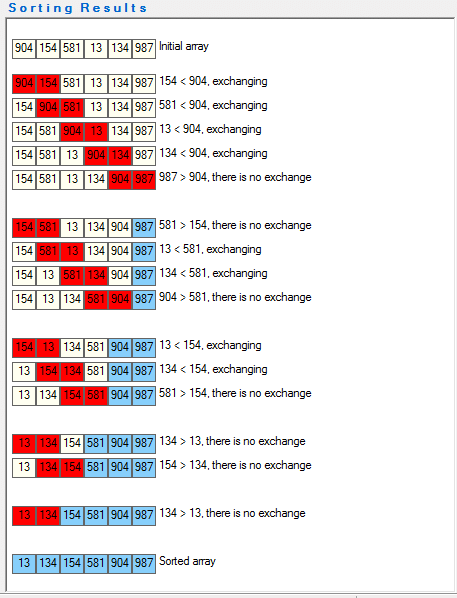
\includegraphics[scale=0.5]{img/Obtained-result-using-Bubble-sort-algorithm-and-array-with-six-elements.png}
    \caption{Corrida de Bubble Sort para un arreglo no ordenado (imagen sacada de Google).}
\end{figure}

A continuación, el código para el algoritmo de la burbuja\marginfootnote{Pseudocódigo sacado del Cormen.}:

\begin{algoritmo}
    \caption{Bubble Sort}\label{alg:bubble}
    \KwData{$A$ arreglo no ordenado}
    \KwResult{$A$ arreglo ordenado}
    \For{$i \leftarrow 1$ \textup{hasta} $length[A]$}{
        \For{$j \leftarrow length[A]$ \textup{hasta} $i+1$}{
        \If{$A[j] < A[j-1]$}{
        intercambia $A[j] \rightleftarrows A[j-1]$
        }
        }
    }
\end{algoritmo}

\break

Analicemos el algoritmo. Las operaciones son comparaciones e intercambio de valores. Así que, si el conjunto tiene $n$ elementos y esa es la medida de la instancia:

\begin{itemize}
    \item Para cada $j$ se hacen $n - j - 1$ comparaciones.
    \item Son $(n-1) + (n-2) + \dots + 2 + 1 = \frac{1}{2}n(n-1)$.
    \item Esto es $O(n^2)$.
    \item La cantidad de intercambios es también $O(n^2)$ (esto en el peor de los casos, se hace un intercambio después de cada comparación).
\end{itemize}

\textbf{En conclusión:} El algoritmo de la burbuja tiene eficiencia $O(n^2)$ en función de la cantidad de elementos del conjunto a ordenar.

Comparemos el algoritmo de la burbuja con una versión del algoritmo de inserción. El \textbf{algoritmo de inserción} construye una lista comenzando con el primer elemento del conjunto dado. Luego agrega el segundo elemento a la lista \textit{en el lugar correcto}. Y así sigue con los demás elementos del conjunto de manera que cada lista queda ordenada de una vez. La eficiencia de este algoritmo depende del método que se utilice para insertar el elemento \textit{en el lugar correcto}.

En nuestro caso, usaremos el método de \textbf{bisección}: Para insertar el $i$-ésimo elemento, se decide en cuál mitad de la lista debería ir. Después, en cuál mitad de esa mitad debería ir y así sucesivamente.

Ahora, analicemos este algoritmo:

\begin{itemize}
    \item Supongamos que el conjunto a ordenar tiene $n$ elementos.
    \item Si $n$ está entre $2^{r-1}$ y $2^r$, entonces hay que hacer $r$ comparaciones.
    \item En total son $\log_22 + \log_23 + \dots + \log_2 n$ comparaciones (aprox.).
    \item Esto es $O(n\log n)$.
\end{itemize}

\textbf{En conclusión}: El algoritmo de inserción, usando el método de bisección tiene eficiencia $O(n \log n)$. Pero al hacer la inserción en el lugar correcto, en el peor de los casos hay que intercambiar los términos de la lista. Esto serían otra vez $n^2$ intercambios. Por tanto, este algoritmo tiene también eficiencia $O(n^2)$.
Lo que hemos hecho es probar un caso particular de un resultado que se le debe a F.P Ramsey. Enunciemos el teorema de Ramsey de la siguiente manera:

\begin{teo}[Ramsey (TR)]\label{teo:TR}
    Para todo $n \in \N$ y todo $k \in \N$
    
    \[
    \omega \rightarrow (\omega)_r^n
    \]
\end{teo}

\begin{proof}
    Procedamos igual que en la demostración anterior con un argumento inductivo: El caso $r=1$ es trivial, así que pasemos a demostrar el caso $r=2$ con inducción sobre $n$.
        
    Si $n=1$, nuevamente es trivial; si $n=2$, ya hemos hecho la demostración en \ref{pre:ramsay1}. Supongamos entonces que el teorema vale para $n$ y probemos para $\omega \rightarrow (\omega)_2^{n+1}$. Como $\N$ es un conjunto infinito numerable, estudiar sus coloraciones vale para cualquier conjunto infinito numerable, así que por conveniencia nos quedaremos estudiando $\N$. Luego, tendremos $f: \N \rightarrow 2$, y nuestro objetivo será conseguir un conjunto homogéneo para $f$.
    
    \begin{marginfigure}
        \centering
        \begin{forest}
            [$0$, for tree={grow=90}, red
                [$1$, red
                    [\vdots
                        [$n-1$, red
                            [$X_1$
                                [$Y_3$
                                    [\vdots]
                                ]
                                [$Y_2$
                                    [\vdots]
                                ]
                            ]
                            [$X_0$
                                [$Y_1$
                                    [\vdots]
                                ]
                                [$Y_0$
                                    [\vdots]
                                ]
                            ]
                        ]
                    ]
                ]
            ]
        \end{forest}
        \caption{Representación de la construcción del árbol construído en la demostración del teorema de Ramsey.}
        \label{fig:ramseyfig1}
    \end{marginfigure}
    
    Entonces, construyamos un árbol de la siguiente manera: Sabemos que los primero $n$ elementos tienen el mismo color, es decir $f(n-1) = i$, donde $i = 0$ o $i = 1$. Definamos entonces dos particiones de $\N$, $X_0$ y $X_1$ tales que
    
    \[
    t \in X_i \iff f\left( n \cup \{t\} \right) = i, \quad i \in \{0,1\}
    \]
      
    \noindent ahora, partiremos ambos conjuntos $X_0$ y $X_1$ de la siguiente manera: Sea $t_0 \in X_0$ el menor elemento de $X_0$ y consideremos $C_{t_0} = \pred(t_0) \cup \{t_0\}$, definiremos dos conjuntos $Y_0$ y $Y_1$ tales que
    
    \[
    t \in Y_i \iff f\left( x \cup \{t\} \right) = i, \quad \forall x \in C_{t_0}^{[n]}
    \]
    
    Supongamos que en este árbol que hemos estado construyendo, tenemos en el nivel $m$ a un elemento $s$, ¿cómo es la partición del conjunto al que pertenece?. Pues consideremos $C_{s} = \pred(t_0) \cup \{s\}$ y sean entonces $Z_0$, $Z_1$ dichas particiones definidas de esta manera:
    
    \[
    t \in Z_i \iff f\left( x \cup \{t\} \right) = i, \quad \forall x \in C_{s}^{[n]}
    \]
    
    Los sucesores inmediatos de $s$ son elegidos de tal forma que tomamos el menor de cada $Z_i$. Entonces cada elemento del nivel $m$ tiene a lo sumo $2^{\binom{m}{n}}$ sucesores inmediatos, ya que para cada elemento del nivel $m$, $\left| C_s^{[n]} \right| = \binom{m}{n}$ y tenemos 2 colores.
    
    Para cada uno de los pares de particiones que hemos construído, puede ocurrir que uno de ellos sea vacío, pero no que los dos sea vacío. Esto es así por la cardinalidad de $\N$.
    
    Como resultado, hemos construído inductivamente un árbol $T$ infinito donde cada nivel es finito, entonces por el teorema \ref{teo:arboles1}, existe una rama $R \subset T$ infinita. Ahora, sea $x \in R^{[n]}$, para todo $s > n$, $t > s$, por construcción tenemos que
    
    \[
    f\left(x \cup \{s\}\right) = f\left(x \cup \{t\}\right)
    \]
    
    Con esto, podemos definir una nueva partición $g: R^{[n]} \rightarrow 2$, donde
    
    \begin{gather*}
        g(x) = 0, \quad \text{si} \quad f(x) = 0 \\
        g(x) = 1, \quad \text{si} \quad f(x) = 1
    \end{gather*}
    
    Luego, recordemos que por hipótesis inductiva, $\omega \rightarrow (\omega)_2^{n}$ y $g$ cumple las condiciones para la hipótesis inductiva. De esta manera, hay un $H \subset R$ infinito tal que $H^{[n]}$ es monocromático para $g$, y por lo tanto monocromático para $f$.
    
    De esta forma, hemos demostrado el caso $r=2$. Supongamos ahora que el teorema es válido para $r \leq k$, es decir que $\omega \rightarrow (\omega)_r^n$ es válido para todo $n$. Sea ahora $f: \N^{[n]} \rightarrow k+1$, podemos definir otra partición auxiliar $G: \N^{[n]} \rightarrow 2$ definida como
    
    \begin{gather*}
        G(x) = 0, \quad \text{si} \quad f(x) = 0 \\
        G(x) = 1, \quad \text{si} \quad f(x) = 1
    \end{gather*}
    
    \noindent entonces, por hipótesis inductiva, $G$ tiene un conjunto homogéneo $H$ infinito. Si $G\left( H^{[n]} \right) = 0$, $H$ es homogéneo para $f$. Si $G\left( H^{[n]} \right) = 1$, entonces $f|H^{[n]}$ es una partición de $k$ partes, y por hipótesis inductiva existe un conjunto $H' \subseteq H$ tal que es infinito y homogéneo. Este conjunto $H'$ también es homogéneo para $f$.
\end{proof}

Con esto demostrado, podemos pasar a demostrar una consecuencia de carácter finita del teorema de Ramsey:

\begin{teo}[Teorema de Ramsey finito (TFR)]\label{teo:TRF}
    Dados números enteros positivos $n, r$ y $m$, existe un entero positivo $N$ tal que
    
    \[
    N \rightarrow (m)_r^n
    \]
\end{teo}

\marginnote{La versión que se usará durante el transcurso del curso es la verión infinita del \TR}.

\begin{proof}
    Supongamos que el teorema no se cumple, es decir que para cada $N \in \N$, existe una coloración $f_N: N^{[n]} \rightarrow k$ tal que $\forall x \in N^{[m]}$, $x^{[n]}$ \textbf{no} es homogéneo para $f_N$.
    
    Con esto, definamos una función $f: \N^{[n+1]} \rightarrow k$ tal que para cualquier sucesión de números naturales $\{a_0, a_1, \dots, a_n\}$ tenemos
    
    \[
    f\left( \{a_0, a_1, \dots, a_n\} \right) = f_{a_n} \left( \{a_0, a_1, \dots, a_{n-1}\} \right)
    \]
    
    \noindent es decir, $f$ asigna a una sucesión creciente de $n+1$ elementos, la coloración será la que le asigne $f_{a_n}$ a los primeros $n$ elementos de esa lista.
    
    Luego, el \hyperref[teo:TR]{TR} nos dice que existe un $H \subset \N$ infinito tal que $H$ es homogéneo para $f$, con $H = \{h_0, h_1, \dots \}$. De esta forma, un conjunto $h$ de $m$ elementos tal que $h \subset H$ es también homogéneo para $f_{h_m}$. Al hacer la restricción $f_N|f_{h_m}$, tenemos que $h$ es homogéneo. Esto es una contradicción, ya que habíamos supuesto que no hay homogéneos de tamaño $m$ para $f_N$.
    
    Por lo tanto, el teorema de Ramsey finito es cierto.
\end{proof}
% Aquí empieza la clase 4

\begin{teo}[Teorema de la función implícita, generalización de la versión 3]
    Sea $F: \R^{n+m} \rightarrow \R^m$ diferenciable y de clase $C^2$, donde $F = (F_1, \dots, F_m)$ y a su vez $F_i(x_1, \dots, x_n, z_1, \dots, z_m)$. Consideremos $p_0 = (x_0, z_0) \in \R^{n+m}$. Consideremos también para cada $i = 1, \dots m$, $\Delta$ de la siguiente manera
    
    \[
    \Delta =
    \renewcommand\arraystretch{2}
    \begin{vmatrix}
        \frac{\partial F_1}{\partial z_1} & \dots & \frac{\partial F_1}{\partial z_m} \\
        \vdots & \ddots & \vdots \\
        \frac{\partial F_m}{\partial z_1} & \dots & \frac{\partial F_m}{\partial z_m}
    \end{vmatrix}
    \]
    
    \noindent donde cada derivada está evaluada en el punto $p_0$.
    
    Si tenemos que $F(p_0) = 0$ y $\Delta(p_0) \neq 0$, entonces en un entorno de $p_0$ tendremos que el sistema
    
    \[
    \begin{cases}
        F_1(x_1, \dots, x_n, z_1, \dots, z_m) = 0 \\
        \vdots \\
        F_m(x_1, \dots, x_n, z_1, \dots, z_m) = 0
    \end{cases}
    \]
    
    \noindent define de forma implícita a las funciones $z_i = f_i(x_1, \dots, x_n)$ con $i = 1, \dots, m$.
    
    Además, tendremos para $k = 1, \dots, n$ y $j = 1, \dots, m$
    
    \[
    \dfrac{\partial z_j}{\partial x_k} = -\dfrac{\dfrac{\partial(F_1, \dots, F_m)}{\partial(z_1, \dots, z_{j-1}, x_k, \dots, z_m)}}{\dfrac{\partial(F_1, \dots, F_m)}{\partial(z_1, \dots, z_m)}}
    \]
\end{teo}

A continuación no demostraremos este último teorema porque los cálculos se hacen muy extensos, pero si discutiremos algunas aplicaciones del T.F.I.:

\begin{ejem}
    Sean una función $F: \R^3 \rightarrow \R$ y $p_o = (x_0, y_0, z_0)$ tal que $F(p_0) = 0$. Sean también $\partial_xF$, $\partial_yF$ y $\partial_zF$ continuas en un entorno de $p_0$. Entonces $F(x,y,z) = 0$ define implícitamente $z = f(x,y)$. Más aún, se puede decir que
    
    \[
    \frac{\partial z}{\partial x}(p_0) = - \frac{\partial_xF(p_0)}{\partial_zF(p_0)}
    \qquad
    \frac{\partial z}{\partial y}(p_0) = - \frac{\partial_yF(p_0)}{\partial_zF(p_0)}
    \]
    
    \noindent si $\partial_zF(p_0) \neq 0$.
    
    Entonces, si calculamos la ecuación del plano tangente, esta nos queda como
    
    \begin{align*}
        z - z_0 &= \frac{\partial f}{\partial x}(x_0,y_0)(x-x_0) + \frac{\partial f}{\partial y}(x_0,y_0)(y-y_0) \\
            &= \partial_zF(p_0)(z-z_0) + \partial_yF(p_0)(y-y_0) + \partial_xF(p_0)(x-x_0) = 0
    \end{align*}
\end{ejem}

\begin{ejem}
    También es muy utilizado en el estudio de las ecuaciones diferenciales ordinarias exactas. Este tema lo abordaremos más adelante.
\end{ejem}

\subsection{Teorema de la función inversa}
\stepcounter{subsec}

Este teorema al igual que el teorema de la función implícita es central en el curso de análisis. Se irá desarrollando poco a poco porque la demostración es bien extensa.

Primero, veremos un lema que además de ser muy útil para la demostración de este teorema, también se utiliza en la materia de ecuaciones diferenciales.

\begin{lem}[Lema de contracción]\label{lem:4.1.1}
    Sean $M \subseteq \R^n$ cerrado y $F: M \rightarrow M$ una función y $K \in (0,1)$ tales que
    
    \[
    \normaeuc{F(x) - F(y)} \leq K\normaeuc{x - y} \quad \forall x,y \in M
    \]
    
    Entonces $F$ tiene un $x_0 \in M$ tal que $F(x_0) = x_0$. Luego nos queda que la sucesión $\sucinf{F^n(x_0)}{n}$ es de Cauchy y converge a $x_0$.
\end{lem}

\begin{proof}
    Primero tenemos que por hipótesis, para cada $x \in M$ fijo y arbitrario
    
    \[
    \normaeuc{F^2(x) - F(x)} = \normaeuc{F(F(x)) - F(x)} \leq K\normaeuc{F(x) - x}
    \]
    
    Ahora, por inducción podemos decir que
    
    \[
    \normaeuc{F^{n+1}(x) - F^n(x)} \leq K\normaeuc{F^n(x) - F^{n-1}(x)} \leq K^n\normaeuc{F(x) - x}
    \]
    
    En lo particular esto nos dice que $\sucinf{F^n(x_0)}{n}$ es una sucesión acotada, ya que
    
    \begin{align*}
        \normaeuc{F^n(x) - x} &\leq \normaeuc{F^n(x) - F^{n-1}(x)} + \normaeuc{F^{n-1}(x) - F^{n-2}(x)} + \dots \normaeuc{F(x) - x} \\
            &\leq \LaTeXunderbrace{(K^{n-1} + K^{n-2} + \dots + K)}_{\text{converge a $\frac{1}{1-K}$}}\normaeuc{F(x) - x}
    \end{align*}
    
    Nuevamente por inducción tenemos que para $m,k \in \N$
    
    \[
    \normaeuc{F^{m+k}(x) + F^m(x)} \leq K^m\normaeuc{F^k(x) + x}
    \]
    
    Ahora, como el término $F^k(x) - x$ está acotado, entonces existe $N_0 \in \N$ tal que $n,m \geq N_0$ con $n = m+k$, entonces
    
    \[
    \text{si $m,m \geq N_0$} \quad \implies \quad \normaeuc{F^{m+k}(x) + F^m(x)} < \varepsilon
    \]
    
    \noindent esto lo podemos hacer porque $\limtoinfty{m}{k^m} = 0$ ya que $K \in (0,1)$.
    
    Por lo tanto, $\sucinf{F^n(x_0)}{n}$ es de Cauchy.
    
    Ahora sea $x_0 \in M$ tal que $x_0 = \limtoinfty{n}{F^n(x)}$. Entonces dado $\varepsilon > 0$, existe $N_1$ tal que
    
    \[
    \text{si $n \geq N_1$} \quad \implies \quad \normaeuc{x_0 - F^n(x)} < \varepsilon
    \]
    
    Por lo tanto, si $n \geq N_1$
    
    \[
    \normaeuc{F(x_0) - F^{n+1}(x)} \leq K\normaeuc{x_0 - F^n(x)} < K\varepsilon
    \]
    
    De esta manera, $\limtoinfty{n}{F^n(x)} = F(x_0)$. En consecuencia $F(x_0) = x_0$.
    
    Lo único que queda es ver que $x_0$ es único: Supongamos que existe $x_1 \in M$ tal que $F(x_1) = x_1$. Consideremos ahora lo siguiente
    
    \begin{align*}
        \normaeuc{x_0 - x_1} &= \normaeuc{F(x_0) - F(x_1)} \leq K\normaeuc{x_0 - x_1} \\
        &\implies \normaeuc{x_0 - x_1} < K\normaeuc{x_0 - x_1}
    \end{align*}
    
    \noindent con $K \in (0,1)$. Esto es una contradicción ya que $\normaeuc{x_0 - x_1} > K\normaeuc{x_0 - x_1}$. Luego no existe dicho $x_1$ y concluimos que $x_0$ es único.
    
    Y así queda demostrado el lema de contracción, que próximamente utilizaremos para la demostración del lema de la función implícita.
\end{proof}

Ahora podemos presentar el teorema de la función inversa. Recordar que de este teorema existen muchas versiones. En este curso nos centraremos en una sola.

\begin{teo}[Teorema de la función inversa]\label{teo:inversa}
    Sean $A \subset \R^n$ abierto, conexo y convexo. Sea $p_0 \in A$, $F: A \rightarrow \R^n$ de clase $C^1(A)$. Supongamos que $JF(p_0) \neq 0$.
    
    Entonces $F$ es $C^1$ invertible localmente en un entorno de $p_0$ y si $G$ es su inversa local, tenemos que $y = G(x)$ y $JG(y) = [JF(x)]^{-1}$.
\end{teo}

\begin{figure}
    \centering
    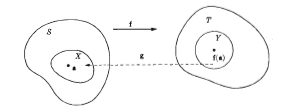
\includegraphics{img/funcion-inversa.PNG}
    \caption{Situación descrita en el teorema de la función inversa.}
\end{figure}

\begin{proof}
    Primero, denotaremos
    
    \[
    \lambda = JF(p_0)
    \]
    
    \noindent así, $\lambda$ define una transformación de $\R^n \rightarrow \R^n$ lineal, continua e invertible. 
    
    Sea ahora $\lambda^{-1} \cdot F(x)$\marginfootnote{No confundir, esto se refiere a la composición.}, derivando nos queda que
    
    \[
    \left( \lambda^{-1} \cdot F(x) \right)' = \lambda^{-1}JF(x)
    \]
    
    \noindent y si $x = p_0$ entonces
    
    \[
    \lambda^{-1}JF(p_0) = \lambda^{-1}\lambda = id
    \]
    
    Entonces, si obtenemos que $\lambda^{-1} \cdot F$ es localmente invervtible, concuimos que $F$ también lo es (ya que $F = \lambda\lambda^{-1}F$). Esto reduce el teorema al caso en que $JF(p_0) = id$.
    
    Sea ahora $q_0 = F(p_0)$ y $H(x) = F(x + p_0) - q_0$ (vemos que $H(0) = 0$). Por lo tanto, $H$ está definida en un abierto que contiene al valor $0$, ya que $F$ está definida en un abierto que contiene a $p_0$. Entonces bastará demostrar que $H$ es invertible (localmente) alrededor de $0$.
    
    Bajo todas estas consideraciones, bastará demostrar el teorema bajo tres simplificaciones relevantes:
    
    \[
    p_0 = 0, \qquad F(0) = 0, \qquad JF(0) = id
    \]
    
    % Aquí empieza la clase 5
    Sea $W(x) = x - F(x)$ donde $JW(x) = I - JF(x)$. Vemos que $JW(0) = 0$. Por continuidad de $F$, existe un valor $r > 0$ tal que
    
    \begin{equation}\label{eq:5.1.1}
        \text{si $\normaeuc{x} < 2r$} \quad \implies \quad \normap{JW(x)}{} \leq \frac{1}{2}
    \end{equation}
    
    \noindent donde $\normap{JW(x)}{} = \sup_{\normaeuc{u} \leq 1} \normaeuc{JW(x) \cdot u}$.
    
    Consideremos ahora $\psi(t) = W(c(t))$, donde $c(t) = tx + (1-t)0$ con $t \in [0,1]$ (en $c(0) = 0$ y en $c(1) = x$). Con esta parametrización, podemos aplicar \TVM~y existe $t_0 \in (0,1)$ tal que
    
    \begin{equation}\label{eq:5.1.2}
        \psi'(t_0) = \psi(1) - \psi(0)
    \end{equation}
    
    Ahora, por un lado tenemos que
    
    \[
    \psi'(t) = JW\left(c(t)\right)x \implies \psi'(t_0) = JW\left(c(t_0)\right)x
    \]
    
    Entonces $\psi(1) = W(x)$ y $\psi(0) = W(0) = 0$. Y por \ref{eq:5.1.1} y \ref{eq:5.1.2} tenemos que
    
    \begin{align*}
        \normaeuc{\psi(t_0)} &\leq \normaeuc{x}\normap{JW\Big( c(t_0) \Big)}{} \\
            &\leq \frac{\normaeuc{x}}{2}
    \end{align*}
    
    Esto nos permite concluir que $\normaeuc{W(x)} \leq \normaeuc{x}/2$. ¿Qué nos está diciendo esto? Que $W$ está definida de esta manera
    
    \[
    W: \overline{B(0,r)} \rightarrow \overline{B(0,r/2)} \quad \text{y} \quad W\left( B(0,r) \right) = B(0, r/2)
    \]
    
    Con la función así definida, ahora queremos asegurar que para dado $y \in \overline{B(0, r/2)}$, existe un único $x \in \overline{B(0,r)}$ tal que $F(x) = y$. Sea ahora $W_y(x) = y + W(x)$. Entonces aplicando nuevamente el \TVM~tendremos lo siguiente:
    
    \begin{align*}
        \normaeuc{W_y(x_1) - W_y(x_2)} &= \normaeuc{y + W(x_1) - y - W(x_2)} = \normaeuc{W(x_1) - W(x_2)} \\
            &\leq \frac{1}{2}\normaeuc{x_1 - x_2}
    \end{align*}
    
    \noindent con $x_1, x_2 \in \overline{B(0,r)}$. Al igual que antes, esto lo logramos con la ayuda de una función auxiliar $\psi(t) = W\left( c(t) \right)$ donde $c(t) = (1-t)x_1 + tx_2$ (con $t \in (0,1)$).
    
    De esta forma, estamos concluyendo que
    
    \[
    \normaeuc{W_y(x_1) - w_y(x_2)} \leq \frac{1}{2} \normaeuc{x_1 - x_2}, \qquad \forall x_1, x_2 \in \overline{B(0,r)}
    \]
    
    Y aplicando el \LC~, se sigue que $W_y$ tiene un único punto fijo $x$ tal que $W_y(x) = x$. Entonces esto implica que
    
    \begin{align}
        x = y + W(x) \quad &\implies \quad x = y + x - F(x) \\
            &\implies \quad F(x) = y
    \end{align}
    
    \noindent para un único valor $x \in \overline{B(0,r/2)}$.
    
    Ahora demostremos la otra parte del teorema. Consideremos el conjunto abierto
    
    \[
    U_1 = \{ x \in B(0,r) : \normaeuc{F(x)} < r/2\}
    \]
    
    Sea $V_1 = F(U_1)$. Así, $F: U \rightarrow V_1$ es inyectiva y podemos construir $G$ tal que $G: V_1 \rightarrow U_1$. Queremos ahora asegurar que $V_1$ es abierto y $G \in C^1$: Sea $x_1$ tal que $y_1 = F(x_1)$ con $\normaeuc{y_1} < r/2$. Sea también $y \in \R^n$ tal que $\normaeuc{y} < r/2$. Entonces hay un único $x \in \overline{B(0,r)}$ tal que $F(x) = y$ y expresando $x = x - F(x) - F(x)$, tendremos que
    
    \begin{align*}
        x - x_1 &= x - F(x) + F(x) - x_1 + F(x_1) - F(x_1) \\
            &= F(x) - F(x_1) + W(x) - W(x_1)
    \end{align*}
    
    Y tomando la norma, nos queda por desigualdad triangular lo siguiente
    
    \begin{align*}
        \normaeuc{x - x_1} &\leq \normaeuc{F(x) - F(x_1)} + \normaeuc{W(x) - W(x_1)} \\
            &\leq \normaeuc{F(x) - F(x_1)} + \frac{\normaeuc{x - x_1}}{2}
    \end{align*}
    
    De aquí obtenemos la siguiente desigualdad
    
    \begin{equation}\label{eq:5.1.3}
        \frac{\normaeuc{x-x_1}}{2} \leq \normaeuc{F(x_1) - F(x_2)}
    \end{equation}
    
    Así, si $y, y_1$ son cercanos entonces $x, x_1$ son también son cercanos. Por lo tanto, tenemos que por un lado
    
    \[
    \normaeuc{x} < r \wedge \normaeuc{F(x)} < \frac{r}{2} \quad \implies \quad x \in U_1 \text{~y por lo tanto $y \in V_1$}
    \]
    
    Esto nos dice que $B(0, r/2) \subset V_1$ y esto implica que $V_1$ es abierto en $\R^n$.
    
    Por otro lado, la desigualdad \ref{eq:5.1.3} implica que
    
    \[
    \frac{\normaeuc{G(y) - G(y_1)}}{2} \leq \normaeuc{y_1 - y}
    \]
    
    Y ahora se puede decir lo siguiente: Dado $\varepsilon > 0$, existe $\delta > 0$ tal que si $\delta > \varepsilon / 2$ entonces concluimos que $G$ es continua.
\end{proof}
\section{Teorema Fundamental del Cálculo y sus aplicaciones}

Ahora, desarrollaremos los resultados para establecer el Teorema Fundamental del Cálculo (TFC). Este teorema fue establecido por Leibniz y es el resultado que nos permite relacionar la teoría de derivadas con la teoría de integración. Este es el teorema central de la teoría de integración.

\begin{lem}
    Sea $f: [a,b] \rightarrow \R$ y $c \in (a,b)$. Si $f$ es integrable en $[a,c]$ y $[c,b]$ entonces $f$ es integrable en $[a,b]$.
\end{lem}

\begin{proof}
    Como la función es integrable en $[a,c]$, dado $\varepsilon > 0$, entonces existe una partición $P_1$ tal que
    
    \[
    U(f, P_1) - L(f, P_1) < \varepsilon/2
    \]
    
    \noindent análogamente, como $f$ es integrable en $[c,b]$, dado $\varepsilon > 0$, existe una partición $P_2$ tal que
    
    \[
    U(f, P_2) - L(f, P_2) < \varepsilon/2
    \]
    
    Ahora, definamos una partición $\Pe = P_1 \cup P_2$, sabemos que esta partición abarca al intervalo $[a,b]$ en su totalidad. Ahora, por \ref{eq:supamasb}, tenemos que
    
    \begin{gather*}
        U(f, \Pe) = U(f, P_1) + U(f, P_2) \\
        L(f, \Pe) = L(f, P_1) + L(f, P_2)
    \end{gather*}
    
    Así, tenemos que
    
    \[
    U(f, \Pe) - L(f, \Pe) = U(f, P_1) - L(f, P_1) + U(f, P_2) - L(f, P_2) < \varepsilon
    \]
    
    \noindent en consecuencia, la función $f$ será integrable en $[a,b]$.
\end{proof}

\begin{teo}
    Sea $f: [a,b] \rightarrow \R$ tal que $f \in \Rint$ y continua en $[a,b]$. Si $F(x) = \int_a^x f(t)dt$ para cada $x \in [a,b]$, entonces $F$\marginfootnote{Establecer esta función nos lleva a la siguiente definición:
    
    \begin{defn}
        Esta función $F$ definida de esta manera se conoce como la \ul{antiderivada} de $f$.
    \end{defn}} es continua en $[a,b]$.
\end{teo}

\begin{proof}
    Sea $\varepsilon > 0$, y los puntos $x_0, x$ en $[a,b]$ ($x > x_0$). Ahora, si queremos ver que $F$ es continua, para dicho $\varepsilon$ hemos de encontrar un $\delta$ tal que se satisfaga lo siguiente:
    
    \[
    \text{si} \quad |x - x_0| < \delta, \qquad \text{entonces} \quad |F(x) - F(x_0)| < \varepsilon
    \]
    
    Ahora, por el lema que acabamos de demostrar, y el teorema \ref{teo:riemod} tenemos
    
    \begin{align*}
        |F(x) - F(x_0)| &= \left| \int_a^x f(t)dt - \int_a^{x_0} f(t)dt \right| = \left| \int_a^x f(t)dt - \int_a^{x_0} f(t)dt \right| \\
        &= \left| \int_a^{x_0} f(t)dt + \int_{x_0}^x f(t)dt - \int_a^{x_0} f(t)dt \right| = \left| \int_{x_0}^x f(t)dt \right| \\
        &\leq \int_{x_0} |f(t)|dt
    \end{align*}
    
    \noindent como $f$ es continua y acotada en $[a,b]$, será acotada en $[x_0, x]$. Por lo tanto existe $M > 0$ tal que
    
    \[
    |F(x) - F(x_0)| \leq M\int_{x_0}^xdt \quad \text{con} \quad \sup_{x\in[a,b]} |f(x)|
    \]
    
    \noindent pero $M\int_{x_0}^xdt = M(x-x_0)$. Entonces, al escoger $\delta = \varepsilon/M$, tendremos que
    
    \[
    |F(x) - F(x_0)| \leq M(x-x_0) \leq M\delta = \epsilon
    \]
    
    De esta manera, queda demostrado.
\end{proof}

\begin{teo}[Primer Teorema Fundamental del Cálculo]\label{teo:1TFC}
    Sea una función $f: [a,b] \rightarrow \R$ con $f \in \Rint$ y continua. Entonces
    
    \[
    F(x) = \intab f(x)dx \quad \text{es derivable}
    \]
    
    Mas aún, $F'(x) = f(x)$.
\end{teo}

\begin{proof}
    En un principio, por definición,
    
    \[
    F'(x) = \lim_{x \to x_0} \frac{F(x) - F(x_0)}{x_0}
    \]
    
    \noindent es decir, que dado $\delta > 0$, queremos hallar un $\varepsilon > 0$ tal que
    
    \[
    \text{si} \quad |x - x_0| < \delta \quad \text{entonces} \left| \frac{F(x) - F(x_0)}{x-x_0} - f(x_0) \right| < \varepsilon
    \]
    
    \noindent entonces, estimemos cuánto da este último factor
    
    \[
    \left| \frac{F(x) - F(x_0)}{x-x_0} - f(x_0) \right| = \left| \frac{F(x) - F(x_0) - f(x_0)(x-x_0)}{x-x_0} \right|
    \]
    
    Por la definición de $F$, y el lema que acabamos de demostrar, tenemos
    
    \[
    \left|\dfrac{F(x) - F(x_0) - f(x_0)(x-x_0)}{x-x_0}\right| = \dfrac{\left| \int_{x_0}^x f(t)dt - \int_{x_0}^x f(x_0)dt  \right|}{|x-x_0|} \leq \dfrac{\int_{x_0}^x |f(t)dt - f(x_0)|}{|x-x_0|}
    \]
    
    Ahora, por la continuidad de $f$, dado $\epsilon > 0$, existe un $\delta_f > 0$ tal que si $|x-x_0| < \delta_f$ entonces $|f(x)-f(x_0)| < \epsilon$. Entonces
    
    \[
    \dfrac{\int_{x_0}^x |f(t)dt - f(x_0)|}{|x-x_0|} \leq \frac{\epsilon}{|x-x_0|}\int_{x_0}^xdt = \epsilon
    \]
    
    Por lo tanto, concluímos que si $|x-x_0| < \delta_f$, tenemos que
    
    \[
    \left| \frac{F(x) - F(x_0)}{x-x_0} - f(x_0) \right| < \varepsilon
    \]
    
    De esta manera, basta fijar $\delta = \delta_f$ para concluir que $F'(x_0) = f(x)$. Y así queda demostrado el teorema.
\end{proof}

\begin{teo}[Segundo Teorema Fundamental del Cálculo]\label{teo:2TFC}
    Sean $f \in C[a,b]$, $F$ tal que $F'(x) = f(x)$. Entonces
    
    \[
    \intab f(x)dx = F(b) - F(a)
    \]
\end{teo}

\begin{proof}
    Sea $G(x) = \int_a^x f(t)dt$, y por el 1TFC, obtenemos que $G'(x) = f(x)$. Pero por otro lado, también tenemos que $F'(x) = f(x)$. Como $G'(x) = F'(x)$ entonces
    
    \[
    G(x) - F(x) = k, \quad \text{con } k \in \R
    \]
    
    \noindent pero sabemos a qué equivale $G$, luego
    
    \[
    \int_a^x f(t)dt - F(x) = k \implies \cancelto{0}{\int_a^af(t)dt} - F(a) = k \implies -F(a) = k
    \]
    
    De esta manera,
    
    \begin{align*}
        \int_a^x f(t)&dt - F(x) = -F(a) \implies \intab f(t)dt - F(b) = -F(a) \\
        &\implies \intab f(t)dt = F(a) - F(b)
    \end{align*}
    
    \noindent y así queda demostrado el teorema.
\end{proof}

La primera aplicación importante que veremos de estos teoremas es una bastante usada en los cursos de cálculo:

\begin{teo}[Cambio de Variable]
    Sean $I_1, I_2 \subset \R$, y sean $f: I_1 \rightarrow I_2$ tal que $f \in C^1(I_1)$\marginfootnote{Aquí estamos manejando la siguiente notación:
    
    \begin{nota}
        Sea $f$ una función, e $I$ un intervalo cualquiera. Decir que $f \in C^1(I_1)$ equivale a pedir que la función sea continua, derivable y que su derivada sea continua sobre el intervalo $I$.
    \end{nota}}, $g: I_2 \rightarrow \R$ tal que $g \in C(I_2)$. Entonces
    
    \[
    \intab g\left(f(t)\right)f'(t)dt = \int_{f(a)}^{f(b)} g(u)du
    \]
\end{teo}

\begin{proof}
    Sea $G$ derivable en $I_2$ tal que $G'(x) = g(x)$. Luego, por 1TFC tenemos que $G(x) = \int_a^x g(u)du$, y por el 2TFC, podemos decir que
    
    \begin{equation}\label{eq:cl6.1}
        G(f(b))-G(f(a)) = \int_{f(a)}^{f(b)} g(u)du \quad \text{porque $G'(x) = g(x)$ para cada $x$}
    \end{equation}
    
    Por otro lado, la regla de la cadena nos dice que
    
    \[
    \left[ G(f(t)) \right]' = G'(f(t))f'(t)
    \]
    
    \noindent entonces, aplicando nuevamente el 2TFC,
    
    \begin{equation}\label{eq:cl6.2}
        \intab \left[ G(f(t)) \right]'dt = G(f(b)) - G(f(a))
    \end{equation}
    
    Luego, por \ref{eq:cl6.1} y \ref{eq:cl6.2} tenemos que
    
    \[
    \int_{f(a)}^{f(b)} g(u)du = \intab \left[ G(f(t)) \right]'dt = \intab g(f(t))f'(t)dt
    \]
    
    De esta forma, queda demostrado.
\end{proof}

\begin{teo}[Integración por partes]
    Sean $f, g \in C^1[a,b]$. Entonces
    
    \[
    \intab f(t)g'(t)dt = f(b)g(b) - f(a)g(a) - \intab f'(t)g(t)dt
    \]
\end{teo}

\begin{proof}
    Sabemos que
    
    \[
    [f(t)g(t)]' = f'(t)g(t) + g'(t)f(t)
    \]
    
    También sabemos por el 2TFC que
    
    \[
    \intab (f(t)g(t))'dt = f(b)g(b) - f(a)g(a)
    \]
    
    Por otro lado,
    
    \[
    \intab (f(t)g(t))'dt = \intab f'(t)g(t)dt + \intab g'(t)f(t)dt
    \]
    
    De esta forma, despejando y sustituyendo nos queda
    
    \begin{gather*}
        \intab g'(t)f(t)dt = \intab (f(t)g(t))'dt - \intab f'(t)g(t)dt \\
        \implies \intab g'(t)f(t)dt = f(b)g(b) - f(a)g(a) - \intab f'(t)g(t)dt
    \end{gather*}
    
    Así, queda demostrado el teorema.
\end{proof}
\subsection{Árboles y algoritmos de ordenamiento}

\begin{defn}
    Una aplicación muy frecuente del teorema \ref{teo:arbol1} es en el estudio de \ul{árboles de desición}, donde cada vértice interno representa una desición y los posibles resultados son representados por los lados. Los resultados finales los representan las hojas del árbol.
\end{defn}

Los algoritmos de ordenamiento revisados anteiormente resuelven el problema al comparar dos enteros y hacer la correspondiente transferencia de datos. Este procedimiento puede representarse como un árbol de desición donde cada vértice representa la comparación entre dos enteros $x$ e $y$, por lo que pueden haber dos resultados posibles, $x < y$ o $x > y$, dando como resultado un árbol binario.

Vimos anteriormente que Bubble Sort \ref{alg:bubble} e Insertion Sort son $O(n^2)$. Ahora veremos un algoritmo llamado \textbf{heapsort}. Este algoritmo es $O(n \log n)$ y hace uso de los árboles para mejorar su eficiencia. Para utilizar este algoritmo, tendremos que representar a los elementos a ordenar como un árbol binario y esto puede hacerse de la siguiente manera:

\begin{marginfigure}
    \centering
    \begin{forest}
    for tree={circle, draw}
    [$x_1$
        [$x_2$
            [$x_4$
                [$x_8$][$x_9$]]
            [$x_5$
                [$x_{10}$]
                [$x_{11}$]]]
        [$x_3$
            [$x_6$
                [$x_{12}$]]
            [$x_7$]]]
    \end{forest}
    \label{fig:pila1}
    \caption{Ejemplo para $n=12$.}
\end{marginfigure}

\vspace{15pt}

\begin{itemize}
    \item Se asignan los miembros de la lista $\{x_1, x_2, \dots, x_n\}$ a ordenar así: Asignamos $x_1$ a la raíz, $x_2$ será el primer hijo de $x_1$ y $x_3$ el segundo, $x_4$ será el primer hijo de $x_2$ y $x_5$ el segundo. Y así sucesivamente.
    \item Siguiendo de esta manera tendremos que el vértice $x_r$ es el padre de $x_{2r}$ y de $x_{2r+1}$. Cuando $n$ es par, el vértice $x_{n/2}$ tiene un único hijo: el vértice $x_n$. Así, hemos construído un árbol binario.
\end{itemize}

Ahora, heapsort tiene dos etapas: Primero, la lista sin ordenar se coloca en un \textit{pila}\marginfootnote{Pasemos a definir una pila:

\begin{defn}
    Una \ul{pila} es una estructura de datos cuya característica principal es que cada padre es menor que sus hijos, es decir que
    
    \[
    x_{2r} < x_{2r} \quad \wedge \quad x_{2r} < x_{2r+1}
    \]
\end{defn}}, y luego dicha pila se transforma en la lista ordenada.

Para la primera etapa, consideremos a los padres en orden inverso: Supongamos que al pararnos en $x_r$, ambos subárboles generados en $x_{2r}$ y $x_{2r+1}$ ya han sido convertidos en pilas. Si $x_r < x_{2r}$ y $x_r < x_{2r+1}$ no hay nada que hacer pues el subárbol que tenemos en $x_{2r}$ ya es una pila. De lo contrario, se intercambian los vértices y se vuelve a comparar e intercambiar para $x_r$ y $x_{4r}$, $x_{4r+1}$. Al llegar a una hoja, ya deberíamos encontrar un sitio donde $x_r$ quede fijo.

Esta regla para formar una pila forma la base para un procedimiento \textbf{pila}$(k,n)$, el cual dado un vértice $x_k$ con la propiedad de que los subárboles con ráiz en $x_{2k}$ y $x_{2k+1}$ son pilas, y hace que el subárbol que parte en $x_k$ sea una pila.

Ahora, en cualquier pila, la raíz siempre tendrá el menor valor, así que va en el primer luegar de la lista ordenada. Luego se sustituye dicho valor en la pila por el de $x_n$, por lo que tendremos un árbol fon $n-1$ vértices donde $x_2$ y $x_3$ son raíces de subárboles que son pilas, por lo que la llamada \textbf{pila}$(1,n-1)$ restaurará la propiedad de pila. Ahora la raíz tiene el menor valor y va en el segundo lugar de la lista ordenada. Y así sucesivamente.

\begin{algoritmo}
    \caption{heapsort}\label{alg:pila}
    \KwData{$\{x_1, \dots, x_n\} \quad$ arreglo no ordenado}
    \KwResult{$\{y_1, \dots, y_n\} \quad$ arreglo ordenado}
    \For{$j \leftarrow 0$ \textup{to} $\lfloor n/2 \rfloor - 1$}{
        \textbf{pila}$(\lfloor n/2 \rfloor - j, n)$
    }
    \For{$i \leftarrow 1$ \textup{to} $n-2$}{
        $y_i \leftarrow x_1; \quad x_1 \leftarrow x_{n-i+1}$ \\
        \textbf{pila}$(1, n-i)$
    }
    $y_{n-1} \leftarrow x_1; \quad y_n \leftarrow x_2$ 
\end{algoritmo}
\section{Clase 8}
\subsection{Resolución de Ecuaciones no homogéneas: Método de Variación de Parámetros}

Antes de pasar a explicar este método, hacen falta un par de teoremas\footnote{La demostración de estos dos teoremas puede encontrarse en el capítulo 3 del Boyce, y son necesarios para los resultados que se establecerán a continuación.} previos:

\begin{teo}
    Si $Y_1$, $Y_2$ son soluciones de la ecuación no homogénea \refeq{eq:edon1}, entonces la diferencia $Y_1 - Y_2$ es una solución a la ecuación homogénea asociada. Más aún, si $y_1$, $y_2$ conforman un conjunto fundamental de soluciones\footnote{Es decir, que $y_1(x)$ y $y_2(x)$ son soluciones a la ecuación y su Wronskiano es distinto de cero.} Entonces

    \[
        Y_1(x) - Y_2(x) = c_1y_1(x) + c_2y_2(x)
    \]

    \noindent con $c_1, c_2$ constantes.
\end{teo}

\begin{teo}
    La solución general de \ref{eq:edon1} puede escribirse en la forma

    \[
        y = \phi(x) = c_1y_1(x) + c_2y_2(x) + Y
    \]

    \noindent donde $y_1, y_2$ conforman un conjunto fundamental de soluciones de la ecuación homogénea asociada, $c_1, c_2$ son constantes, e $Y$ es una solución en específico de \ref{eq:edon1}.
\end{teo}

Recordemos que una ecuación diferencial no homogénea es aquella de la forma \refeq{eq:edon1}. La idea del método de Variación de Parámetros, es encontrar primero una solución a la ecuación homogénea asociada

\[
    y_c(x) = c_1y_1 + c_2y_2 = 0
\]

La idea básica es reemplazar las constantes $c_1$ y $c_2$ por funciones $u_1(x)$, $u_2(x)$ respectivamente, y hallar estas funciones de tal forma que la expresión

\[
    y = u_1y_1 + u_2y_2
\]

Es una solución de \ref{eq:edon1}.

\textbf{(!!!!) Toda esta charla que viene de $y'$ y $y''$ no la entendí muy bien, y tampoco entiendo muy bien qué es lo que se concluye. PREGUNTAR.}

Desarrollando esta idea, derivemos $y$ para hallar $u_1$ y $u_2$ en el proceso:

\begin{equation*}
    \begin{aligned}
        y' &= u_1'y_1 + u_2'y_2 + u_2y_2' + u_1y_1' \\
        y'' &= u_1''y_1 + u_1'y_1' + u_2''y_2 + u_2'y_2' + u_2'y_2' + u_2y_2'' + u_1'y_1' + u_1y_1''
    \end{aligned}
\end{equation*}

Como $y_1$, $y_2$ son soluciones de la ecuación homogénea asociada, Entonces

\[
    u_1'y_1 + u_2'y_2 = 0
\]

Y esto implica que

\begin{equation*}
    \begin{aligned}
        y' &= u_2y_2' + u_1y_1' \\
        y'' &=  u_1'y_1' + u_2'y_2' + u_2y_2'' + u_1y_1''
    \end{aligned}
\end{equation*}

Luego, gracias a los teoremas visto al inicio de la sección, sabemos que

\[
    f(x) = \LaTeXunderbrace{u_1(y_1'' + py_1' + qy_1) + u_2(y_2'' + py_2' + qy_2)}_{\text{Solución a la ecuación homogénea asociada}} + \LaTeXoverbrace{u_1'y_1' + u_2'y_2'}^{\mathclap{\text{Solución específica de la ecuación no homogénea}}}\footnotemark
\]\footnotetext{Como $y_1, y_2$ conforman un conjunto fundamental de soluciones, entonces también $y_1', y_2'$ también conforman uno.}

Como $W(y_1, y_2) \neq 0$, todo esto nos da como resultado el sistema

\begin{equation}
    \begin{cases*}
        u_1'y_1 + u_2'y_2 = 0 \\
        u_1'y_1' + u_2'y_2' = f(x)
    \end{cases*}
\end{equation}

De donde

\[
    u_1' = -\frac{y_2f(x)}{W(y_1, y_2)} \qquad u_2' = \frac{y_1f(x)}{W(y_1, y_2)}
\]

Todo esto nos quiere decir que para resolver EDO de este tipo, basta con seguir los siguientes pasos:

\begin{enumerate}
    \item Calcular $y_c$.
    \item Calcular $W(y_1, y_2)$.
    \item Aplicar $u_1', u_2'$ y calcular sus integrales.
\end{enumerate}
Para este teorema, la hipótesis de convergencia uniforme es clave. Veremos a continuación como en general, el teorema no se cumple para la convergencia puntual.

\begin{ejem}
    Consideremos la siguiente sucesión de funciones sobre $D = [0,1]$:
    
    \[
    f_{n-1}(x) = \begin{cases}
                 2n \quad x \in (1/n, 2/n) \\
                 0  \quad \text{si no}
             \end{cases}
    \]
    
    \noindent con $n \geq 2$.
    
    Al analizar las gráficas, estas son muy parecidas a las de \ref{ejem:cp}, y nos daremos cuenta de que la gráfica tenderá a cero. Entonces
    
    \[
    \limtoinfty{n}{f_n(x)} = f(x) \quad \text{donde $f(x) \equiv 0$ para cada $x \in [0,1]$}
    \]
    
    Pero
    
    \[
    \int_0^1 f_n(x)dx = \int_{\frac{1}{n}}^{\frac{2}{n}} 2ndx = 2
    \]
    
    Por lo tanto $\limtoinfty{n}{\int_0^1 f_n(x)dx} = 2$ y $\int_0^1 \limtoinfty{n}{f_n(x)}dx = 0$.
\end{ejem}

\begin{cor}
    Sea $\sucinf{f}{n}$ una sucesión de funciones integrables en $[a,b]$, y supongamos que $\sumtoinfty{n=1}{f_n}$ c.u. Entonces
    
    \[
    \intab \left(\sumtoinfty{n=1}{f_n(x)}\right)dx = \sumtoinfty{n=1}{\intab f_n(x)dx}
    \]
\end{cor}

\begin{proof}
    Como $\sucinf{f}{n}$ son integrables Riemann-integrables, entonces por las propiedades de la integral de Riemann, $\sucinf{S}{N}$ son integrables. Como $\sumtoinfty{n=1}{f_n}$ c.u entonces existe $f$ tal que
    
    \[
    \limtoinfty{N}{S_N} = f \quad \text{uniformemente}
    \]
    
    Entonces
    
    \[
    \limtoinfty{N}{\intab S_N(x)dx} = \intab f(x)dx
    \]
    
    Y en conclusión,
    
    \[
    \intab \left(\sumtoinfty{n=1}{f_n(x)}\right)dx = \sumtoinfty{n=1}{\intab f_n(x)dx}
    \]
    
    Así, queda demostrado.
\end{proof}

\begin{ejem}
    Consideremos la siguiente sucesión sobre $D = [0,1]$: $f_n(x) = x^n$ con $n \geq 0$. En el ejemplo \ref{ej:x^n} vimos que
    
    \[
    \sumtoinfty{n=0}{x^n} = \frac{1}{1-x} \quad \text{para cada $x \in [0,1]$}
    \]
    
    Consideremos un $r \in [0,1]$ tal que $x < r$. Entonces
    
    \[
    \left| \sumtoinfty{n=0}{x^n} \right| \leq \sumtoinfty{n=0}{|x^n|} < \sumtoinfty{n=0}{r^n} \qquad \footnotemark
    \]\footnotetext{Como ejercicio, se plantea lo siguiente:
    
    \begin{ejer}
        Demostrar que $\left| \sumtoinfty{n=0}{x^n} \right| \leq \sumtoinfty{n=0}{|x^n|}$.
    \end{ejer}}
    
    Ahora, tenemos una serie numérica $\sumtoinfty{n=0}{r^n}$ que converge a $\frac{1}{1-r}$, y por el teorema \ref{teo:wei}, nos queda que $\sumtoinfty{n=0}{x^n}$ converge. Luego, podemos intercambiar integrales por series gracias al corolario que recién establecimos. Así, sea $y \in (0, r)$,
    
    \[
    -\ln(1-y) = \int_0^y \frac{dx}{1-x} = \int_0^y \left( \sumtoinfty{n=0}{x^n}\right)dx = \sumtoinfty{n=0}{\int_0^y x^ndx} = \sumtoinfty{n=0}{\frac{y^{n+1}}{n+1}}
    \]
    
    De esta forma, hemos obtenido el desarrollo en series de $-\ln(1-y)$. De la misma manera podremos obtener el desarrollo en series de muchas funciones elementales.
\end{ejem}

\begin{teo}
    Sea $\sucinf{f}{n} \subset C'[a,b]$\marginfootnote{Recordemos que $C'$ quiere decir que:
    
    \begin{enumerate}
        \item $f_n: [a,b] \rightarrow \R$.
        \item $f_n$ son continuas.
        \item $f'_n$ son continuas.
    \end{enumerate}}. Supongamos que
    
    \begin{itemize}
        \item $f'_n \xrightarrow[n \to \infty]{\text{c.u}} g$.
        \item $f_n \xrightarrow[n \to \infty]{\text{c.p}} g$.
    \end{itemize}
    
    Entonces $f_n \xrightarrow[n \to \infty]{\text{c.u}} f$ y $f' = g$.
\end{teo}

\begin{proof}
    Demostremos ambos puntos en orden:
    
    \begin{itemize}
        \item Por el 2TFC, dados $m,n \in \N$, $x \in [a,b]$, entonces
    
        \[
        f_n(x) - f_m(x) = \int_a^x (f_n - f_m)'(t)dt + (f_n - f_m)(a)
        \]
        
        Luego
        
        \begin{equation}\label{eq:suc1}
            \norma{f_n - f_m} = \sup_{x \in D} \left| f_n(x) - f_m(x) \right| \leq (b-a)\norma{(f_n - f_m)'} + \left| (f_n - f_m)(a) \right| \quad \footnotemark
        \end{equation}\footnotetext{Se sustituye lo que está en la expresión anterior por lo que tenemos en la norma, y se desarrolla para llegar a ese resultado.}
        
        Por otro lado, como $f'_n$ c.u, entonces es fuertemente Cauchy, y además $\limtoinfty{n}{f_n(a)} = f(a)$ por la c.p de $f_n$. Entonces dado $\varepsilon > 0$, existe un $N_1 \in \N$ tal que
        
        \[
        \norma{(f_n - f_m)'} < \frac{\varepsilon}{2(b-a)}
        \]
        
        \noindent y además, existe un $N_2 \in \N$ tal que
        
        \[
        \left| (f_n - f_m)(a) \right| < \frac{\varepsilon}{2}
        \]
        
        \noindent si $n, m \in \N$ tales que $n, m \geq N_0 = \max(N_1, N_2)$.
        
        Ahora, por \ref{eq:suc1} tenemos que
        
        \[
        \norma{f_n - f_m} \leq (b-a)\norma{(f_n - f_m)'} + \left| (f_n - f_m)(a) \right| < \frac{\varepsilon(b-a)}{2(b-a)} + \frac{\varepsilon}{2} = \varepsilon
        \]
        
        De esta forma, dado $\varepsilon > 0$ entonces existe un $N_0$ tal que si $n, m \geq N_0$ entonces $\norma{f_n - f_m} < \varepsilon$. En conclusión, $\sucinf{f}{n}$ cumple la condición de Cauchy, por lo tanto $f_n \xrightarrow[]{\text{c.u}} f$.
        
        \item Por el 2TFC, tenemos que para cada $n \in \N$,
        
        \[
        f_n(x) = \int_a^x f'_n(t)dt - f_n(a)
        \]
        
        De esta manera,
        
        \begin{gather*}
            f(x) = \limtoinfty{n}{f_n(x)} = \limtoinfty{n}{\left[ \int_a^x f'_n(t)dt - f_n(a) \right]} = \limtoinfty{n}{\int_a^x f'_n(t)dt} - \limtoinfty{n}{f_n(a)} \\
            = \int_a^x [\limtoinfty{n}{f'_n(t)}]dt - f(a) = \int_a^x g(t)dt - f(a)
        \end{gather*}
        
        Nuevamente, por el 1TFC lo anterior implica que $f'(x) = g(x)$.
    \end{itemize}
    
    Así, quedan demostrados ambos puntos.
\end{proof}

\begin{cor}\label{cor:poderosisimo}
    Sea $\sucinf{f}{n} \subset C'[a,b]$ tales que:
    
    \begin{enumerate}
        \item $\sumtoinfty{n=1}{f_n}$ c.p.
        \item $\sumtoinfty{n=1}{f'_n}$ c.u.
    \end{enumerate}
    
    Entonces $\sumtoinfty{n=1}{f_n}$ c.u y además
    
    \[
    \left( \sumtoinfty{n=1}{f_n(t)} \right)' = \sumtoinfty{n=1}{f'_n(x)} \quad \footnotemark
    \]\footnotetext{Como ejercicio queda la demostración del corolario \ref{cor:poderosisimo}. La demostración se logra haciendo el mismo argumento que en el teorema anterior, pero definiendo $S_N = f_1 + \dots + f_N$.}
\end{cor}

\subsection{Teorema de Stone-Weierstrass}

\begin{teo}[Stone-Weierstrass]
    Sea $f \in C[a,b]$, entonces existe una sucesión $\sucinf{P}{n}$ de polinomios en $[a,b]$ tal que $\norma{P_n - f} \xrightarrow[n \to \infty]{} 0$.
\end{teo}

\begin{proof}
    Como primera consideración, en lugar de realizar la demostración en $[a,b]$, la realizaremos en $[0,1]$, podemos hacer esto debido a que si consideramos una función $p(x): [a,b] \rightarrow [0,1]$ tal que
    
    \[
    p(x) = \frac{x-a}{b-a}
    \]
    
    \noindent entonces podemos tomar una composición $p \circ f$, donde $f$ está definida en $[a,b]$.
    
    \begin{marginfigure}
        \centering
        \begin{tikzpicture}
            \begin{axis}[
                axis x line = bottom,
                axis y line = left,
                domain=0:1.1,
                width=5cm,
                height=5cm,
                clip=false,
                xtick=\empty,
                ytick=\empty,
                every axis x label/.style={at={(ticklabel cs: 0.95,0)},
                anchor=north},
                every axis y label/.style={at={(ticklabel cs: 0.95,0)},
                anchor=north east},
                xlabel=$x$,
                ylabel=$y$,
                ]
                \addplot [mark=none, blue, smooth] coordinates { (0,0.5) (0.1,0.4) (0.25, 0.2) (0.6,0.6) (0.8,0.3) (1,0.4) };
                \addplot [mark=*, red] coordinates { (0,0.5) (1,0.4) };
                \node[] at (-13,295) {\footnotesize $f(0)$};
                \node[] at (115,200) {\footnotesize $f(1)$};
            \end{axis}
        \end{tikzpicture}
        \label{fig:stnwei1}
        \caption{\footnotesize Aquí describimos la situación que tenemos en la demostración. Tenemos $f(x)$ como la línea azul, y $L(x)$ como la línea roja.}
    \end{marginfigure}
    
    La otra consideración es que $f(0) = f(1) = 0$. Esto lo podemos hacer porque al tomar la recta $L(x)$ que pasa por $f(0)$ y $f(1)$, entonces
    
    \[
    L(x) = (f(1) - f(0))x - f(0)
    \]
    
    \noindent definamos entonces $h(x) = f(x) - L(x)$. Luego, $h(1) = h(0) = 0$. Lo que hemos hecho es transladar la función $f$, obteniendo una nueva función $h(x)$. De esta manera podemos tomar $f(1) = f(0) = 0$.
    
    Sean para $n \in \N$
    
    \[
    K_n(t) = \begin{cases}
        \dfrac{(1-t^2)^n}{C_n}& \quad \text{si} \quad |t| \leq 1 \\
        0& \quad \text{si} \quad |t| > 1
    \end{cases}
    \]
    
    \noindent donde $\displaystyle C_n = \int_{-1}^1 (1-t^2)^ndt$. Como $(1-t^2)^n$ es una función acotada, la integral dará como resultado un valor finito y positivo (ya que $|t| \leq 1$).\marginfootnote{Estos valores se llaman los núcleos de Landau.}
    
    \begin{marginfigure}
        \centering
        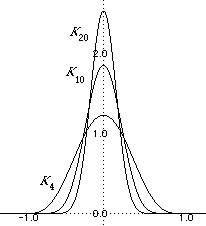
\includegraphics[scale=0.7]{img/landau.png}
        \label{fig:stnwei1}
        \caption{\footnotesize Aquí están representados los núcleos de Landau para algunos valores de $n$.}
    \end{marginfigure}
    
    Sea $z_n(t) = (1-t^2)^n$,
    
    \[
    z_n(-t) = (1-(-t)^2)^n = (1-t^2)^n = z_n(t)
    \]
    
    Por lo tanto, es una función par. Luego
    
    \[
    C_n = \int_{-1}^1 (1-t^2)^ndt = 2\int_0^1 (1-t^2)^ndt \geq 2\int_0^1 (1-t)^ndt = \frac{2}{n+1}
    \]
    
    Por otro lado, si definimos
    
    \[
    P_n(x) = \int_{\R} f(t)K_n(x-t)dt
    \]
    
    Lo primero que podemos notar es que $P_n$ son polinomios, porque $K_n(x-t)$ lo son. Esto es verificable gracias al binomio de Newton. Estimemos entonces cuánto vale $|P_n(x) - f(x)|$
    
    \[
    |P_n(x) - f(x)| = \left| \int_{\R} (f(x) - f(t))K_n(x-t)dt \right|
    \]
    
    \noindent ya que el valor de la integral de los $K_n$ es igual a $1$ \marginfootnote{Esto es porque
    
    \[
    \int_{-1}^1 K_n(t)dt = \frac{1}{C_n} \int_{-1}^1 (1-t^2)^ndt = 1
    \]}. Continuamos desarrollando
    
    \[
    \left| \int_{\R} (f(x) - f(t))K_n(x-t)dt \right| \leq \left| \int_{\R} (f(x) - f(t))\right| K_n(x-t)dt
    \]
    
    Hacemos ahora cambio de variable $u = x-t$. Entonces, lo anterior nos queda como
    
    \[
    \left| \int_{\R} (f(x-u) - f(x))\right| K_n(u)du
    \]
    
    Como $f$ es continua en $[0,1]$, el cual es compacto, entonces $f$ es uniformemente continua. Entonces dado $\varepsilon > 0$, existe un $\delta > 0$ tal que
    
    \begin{equation}\label{eq:stnwei1}
        \text{si} \quad |x-x-u| < \delta \implies |f(x) - f(x-u)| < \varepsilon
    \end{equation}
    
    Entonces, reescribiendo lo que teníamos antes, y separando la integral tenemos que
    
    \begin{gather}\label{eq:stnwei2}
        |P_n(x) - f(x)| \leq \notag \\
        \int_{|u| < \delta/2} \left|f(x-u) - f(x)\right|K_n(u)du + \int_{\delta/2 < |u| < 1} \left|f(x-u) - f(x)\right|K_n(u)du
    \end{gather}
    
    Por un lado, si $|u| < \delta/2$ y se cumple la hipótesis de continuidad, por \ref{eq:stnwei1} tendremos que
    
    \[
    \int_{|u| < \delta/2} \left|f(x-u) - f(x)\right|K_n(u)du \leq \varepsilon \int_{-1}^1 du = \varepsilon
    \]
    
    Y por el otro lado, como $K_n$ son funciones continuas y decrecientes en el intervalo $[\delta/2, 1]$, entonces para $\delta/2 < |u| < 1$, el máximo valor que pueden tomar es $K_n(\delta/2)$. Luego
    
    \begin{gather*}
        \int_{\delta/2 < |u| < 1} \left|f(x-u) - f(x)\right|K_n(u)du \leq K_n(\delta/2)\int_{\delta/2 < |u| < 1} \left|f(x-u) - f(x)\right|du \leq \\
        K_n(\delta/2)\int_{\delta/2 < |u| < 1} 2\norma{f}du = K_n(\delta/2)(2\norma{f})\int_{\delta/2 < |u| < 1}du \leq \\
        K_n(\delta/2)(2\norma{f})\int_{0 < |u| < 1}du = K_n(\delta/2)2\norma{f}
    \end{gather*}
    
    \noindent como los $K_n$ son integrables, conforman una sucesión que converge a cero al hacer $n \rightarrow \infty$. Entonces la expresión $\int_{\delta/2 < |u| < 1} \left|f(x-u) - f(x)\right|K_n(u)du$ puede hacerse tan pequeña como queramos.
    
    De esta forma, retomando lo que teníamos en \ref{eq:stnwei2}
    
    \begin{gather*}
        |P_n(x) - f(x)| < \varepsilon + 0 = \varepsilon \implies \\
        |P_n(x) - f(x)| \xrightarrow[n \to \infty]{} 0 \quad \forall x \in [0,1]
    \end{gather*}
    
    \noindent como el límite es igual a cero cuando $n$ tiene a infinito, pero no depende de $x$, podemos concluir que
    
    \[
    \norma{P_n - f} \xrightarrow[n \to \infty]{} 0
    \]
    
    De esta forma, queda demostrado el teorema.
\end{proof}

\end{document}